\documentclass[main]{subfiles}

\begin{document}

\tableofcontents
\newpage

\section{Lie groups}

\begin{definition}
Let $G$ be a Lie group, the \textit{Lie algebra} $\Lie(G)$ of $G$ can be defined in the following equivalent ways
\begin{enumerate}
\item The vector space of left invariant vector fields
\item The tangent space at the identity $T_eG$
\end{enumerate}
\end{definition}

\begin{definition}
A \textit{one-parameter subgroup} is a group homomorphism $\phi:\mathbb R\to G$
\end{definition}

\begin{proposition}\hfill
\begin{enumerate}
\item Lie groups are parallelizable
\item One parameter subgroups are precisely the maximal integral curves of the left invariant vector fields starting at $e$. So there is a one to one correspondence between One parameter subgroups of $G$ and $\Lie(G)$
\end{enumerate}
\end{proposition}

\begin{proof}
\begin{enumerate}
\item For any $0\neq X_e\in T_eG$, we can define a vector field $X_g=g_*X_e$, this is a nonvanishing global section of the tangent bundle
\item Suppose $\phi:\mathbb R\to G$ is a one parameter subgroup, let $X_e=\phi'(0)$, then we have a left invariant vector field $X$ on $G$, think of $\frac{\partial}{\partial t}$ as a left invariant vector field on $\mathbb R$, thus $\phi$ as Lie group homomorphism induces $\phi_*\frac{\partial}{\partial t}$ which is also a left invariant vector field and $\phi'(s)=(d\phi)_s\left.\frac{\partial}{\partial t}\right|_s=X_{\phi(s)}$. Conversely, if $\phi:\mathbb R\to G$ is the maximal integral curve of some left invariant vector field $X$, suppose the global flow generated by $X$ is $\varphi:G\times\mathbb R\to G$, then $\varphi(e,t)=\phi(t)$, $\phi(t+s)=\varphi(e,t+s)=\varphi(\varphi(e,t),s)=\varphi(\phi(t),s)$, since $L_{\phi(t)}$ is an isomorphism, thus $L_{\phi(t)}\circ\phi$ is the maximal integral curve starting at $\phi(t)$, thus $\varphi(\phi(t),s)=\phi(t)\phi(s)$
\end{enumerate}
\end{proof}

\begin{theorem}[Lie correspondence]\hfill
\begin{enumerate}
\item If $\phi:G\to H$ is a homomorphism of Lie groups, then $d\phi:\Lie(G)\to\Lie(H)$ or $(d\phi)_e:T_eG\to T_eH$ is an homomorphism of Lie algebras. Suppose $H\leq G$ is a Lie subgroup, then $\Lie(H)=T_eH\leq T_eG$
\item $d\phi:\Lie(G)\to\Lie(H)$ or $(d\phi)_1:T_1G\to T_1H$ is an homomorphism of Lie algebras
\end{enumerate}
\end{theorem}

\begin{proof}
\begin{enumerate}
\item 
\item Suppose $X$ is a left invariant vector field on $G$, then $(d\phi)_gX_g=(d\phi)_g(dL_g)_1X_1(f)=X_1(f\circ\phi\circ L_g)=X_1(f\circ\phi\circ L_g)=(dL_{\phi(g)})_1(d\phi)_1X_1(f)$ which gives a left invariant vector field, thus using Lemma \ref{Pushforward of vector field} \begin{align*}
(d\phi)[X,Y](f)&=[X,Y](f\circ\phi) \\
&=X(Y(f\circ\phi))-Y(X(f\circ\phi)) \\
&=X(((d\phi Y)f)\circ\phi)-Y(((d\phi X)f)\circ\phi) \\
&=((d\phi X)(d\phi Y)f)\circ\phi-((d\phi Y)(d\phi X)f)\circ\phi \\
&=([d\phi X,d\phi Y]f)\circ\phi
\end{align*}
Therefore $(d\phi)[X,Y]=[(d\phi X),(d\phi Y)]$, $d\phi$ is a Lie algebra homomorphism
\end{enumerate}
\end{proof}

\begin{proposition}
Suppose $(\pi,V)$ is a complex representation of a compact Lie group $G$, then there exists a positive definite Hermitian form such that this representation is unitary
\end{proposition}

\begin{proof}
Choose any positive definite Hermitian form $\langle,\rangle$, define Hermitian form
\[(v,w):=\displaystyle\int_G\langle gv,gw\rangle d\mu\]
Here $\mu$ is the Haar measure with $\displaystyle\int_G d\mu=1$, $(,)$ is $G$ left invariant
\end{proof}

\begin{definition}
Suppose $G$ acts on $M$, $G_p$ is the stablizer of $p$. The \textit{isotropy representation}\index{Isotropy representation} is $G_p\to GL(T_pM)$
\end{definition}

\begin{example}
Consider Lie group $\SL(2,\mathbb C)$ whose Lie algebra is $\mathfrak{sl}(2,\mathbb C)$, which is generated by $H=\begin{pmatrix}
1&0 \\
0&-1
\end{pmatrix},X=\begin{pmatrix}
0&1 \\
0&0
\end{pmatrix},Y=\begin{pmatrix}
0&0 \\
1&0
\end{pmatrix}$, thus $D_H=-x_1\dfrac{\partial}{\partial x_1}+x_2\dfrac{\partial}{\partial x_2},D_X=-x_2\dfrac{\partial}{\partial x_1},D_Y=-x_1\dfrac{\partial}{\partial x_2}$
\end{example}

\begin{definition}
For any $A\in T_1G$, define the exponential map $\exp A:=\phi_A(1)$ where $\phi_A:\mathbb R\to G$ is the one parameter subgroup corresponding to $A$, also it is easy to see that $\exp tA:=\phi_{tA}(1)=\phi_A(t)$ which is a scaling of the integral curve, and $\exp(t+s)A=\exp tA\exp sA$ since $\exp tA$ is a one parameter subgroup, and thus $(\exp A)^{-1}=\exp(-A)$
\end{definition}

\begin{proposition}(\textit{Properties of exponential map})\label{Properties of exponential map} \par
Let $G,H$ be Lie groups with Lie algebras $\mathfrak{g},\mathfrak{h}$ \par
\textit{(a) }The exponential map is a smooth map \par
\textit{(b) }$(d\exp)_0:\mathfrak g\cong T_0\mathfrak{g}\to T_1G\cong\mathfrak{g}$ is the identity map, which implies that the exponential map is a local diffeomorphism around $0$ \par
\textit{(c) }Suppose $\phi:G\to H$ is a Lie group homomorphism, then the following diagram commutes
\begin{center}
\begin{tikzcd}
\mathfrak{g} \arrow[r,"(d\phi)_1"] \arrow[d,"\exp"] & \mathfrak{h} \arrow[d,"\exp"] \\
G \arrow[r,"\phi"] & H
\end{tikzcd}
\end{center}
\end{proposition}

\begin{proof} $\\$
\textit{(a) } \par
\textit{(b) }For any $A\in\mathfrak{g}$, consider $\gamma:\mathbb R\to\mathfrak g,t\mapsto tA$ which is a one parameter subgroup of $\mathfrak g$, thus $A=\gamma'(0)\in T_0\mathfrak g$, and $\exp A=\gamma(1)=A$ \par
\textit{(c) }Define $\gamma(t)=\phi(\exp tA)$ which is a one parameter subgroup of $H$ since $\gamma(t+s)=\phi(\exp(t+s)A)=\phi(\exp tA\exp sA)=\phi(\exp tA)\phi(\exp sA)=\gamma(t)\gamma(s)$, then $\gamma'(0)=\left.\dfrac{\partial}{\partial t}\right|_{t=0}\phi(\exp tA)=(d\phi)_1\left.\dfrac{\partial}{\partial t}\right|_{t=0}\exp tA=(d\phi)_1A$, on the other hand, $\exp(t(d\phi)_1A)$ is one parameter subgroup of $H$ corresponds to $(d\phi)_1A=\gamma'(0)$, thus $\exp(t(d\phi)_1A)=\gamma(t)=\phi(\exp tA)$
\end{proof}

\begin{proposition}
Let $G$ be a Lie group and $H\leq G$ a Lie subgroup, then $\Lie(H)=\left\{A\in\Lie(G)\middle|\exp tA\in H,\forall t\in\mathbb R\right\}$
\end{proposition}



\section{Lie algebra}

\begin{definition}\index{Nonassociative algebra}
A \textit{nonassociative} $k$-\textit{algebra}\index{Nonassociative $k$ algebra} $A$ is an $k$ vector space with a multiplication $\cdot$ such that it is distributive $(a+b)\cdot c=a\cdot c+b\cdot c$, $a\cdot(b+c)=a\cdot b+a\cdot c$. $A$
\begin{itemize}
\item is \textit{unital} if $1\in A$
\item is \textit{symmetric} if $xy=yx$
\item is \textit{antisymmetric} if $xy=-yx$
\item satisfies \textit{Jacobi identity}\index{Jacobi identity} if $(xy)z+(yz)x+(zx)y=0$
\end{itemize}
A homomorphism $\phi:A\to B$ is a linear map such that $\phi(xy)=\phi(x)\phi(y)$
\end{definition}

\begin{definition}
Suppose $e_1,\cdots, e_n$ is a basis of $A$, $e_ie_j=\displaystyle\sum_ic_k^{ij}e_k$, $c_k^{ij}$ are called \textit{structure constants} with respect to $e_1,\cdots, e_n$. If $A$ satisfies Jacobi identity, then
\[\sum_lc_m^{il}c_l^{jk}+\sum_lc_m^{jl}c_l^{ki}+\sum_lc_m^{kl}c_l^{ij}=0\]
\end{definition}

\begin{definition}
$B\leq A$ is a \textit{subalgebra} if $B$ is a subspace such that $BB\subseteq B$. $I\leq A$ is a \textit{left ideal} if $AI\subseteq I$. Suppose $I,J\leq A$ are ideals, define \textit{ideal quotients} $(J:I)=\{x\in A|xI\subseteq J\}$ which is an ideal. Homomorphisms preserve ideals
\end{definition}

\begin{remark}
If $A$ is (anti)symmetric, left ideals are two-sided ideals
\end{remark}

\begin{definition}
$A$ is \textit{abelian} if $AA=0$, $A$ is \textit{simple} if it is not abelian and the only ideals are $0$ and $A$, $A$ is \textit{semisimple} if $A=A_1\oplus\cdots\oplus A_n$ is the direct sum of simple subalgebras, $A$ is \textit{reductive} if $A=\mathfrak{s}\oplus\mathfrak{a}$ is a direct sum of a semisimple subalgebra $\mathfrak{s}$ and an abelian subalgebra $\mathfrak{a}$
\end{definition}

\begin{definition}
A \textit{derivation}\index{Derivation} is an endomorphism $D:A\to A$ such that $D(ab)=D(a)b+aD(b)$. Derivation algebra $\Der_{k}(A)$ is the set of all derivations. If $D_1,D_2\in \Der_{k}(A)$, then $[D_1,D_2]=D_1D_2-D_2D_1\in \Der_{k}(A)$, $\Der_{k}(A)\leq \End_{k}(A)$ is a Lie subalgebra
\end{definition}

\begin{definition}
$R\xrightarrow\varphi S$ is a ring homomorphism between commutative rings. The module of \textit{K\"ahler differentials}\index{K\"ahler differentials} is $\Omega_{S/R}$ satisfies the universal property that any derivation uniquely factors through $d_{S/R}:S\to\Omega_{S/R}$, i.e. $\Hom_S(\Omega_{S/R},M)\cong\Der_R(S,M)$. $\Omega_{S/R}$ can be constructed as
\[\frac{\{ds:s\in S\}}{dr=0,d(s+t)=ds+dt,d(st)=sdt+tds}\]
Another construction: define $I$ to be the kernel of $S\otimes_RS\to S$, $s\otimes t\mapsto st$, and $\Omega_{S/R}=I/I^2$, with $ds=1\otimes s-s\otimes 1$, the free $S$ module generated by $ds$ consists of $t\otimes s-ts\otimes1$, which is the kernel of $S\otimes_RS\to S\otimes_RR$, $t\otimes s\mapsto ts\otimes 1$, moding $I^2$ is precisely the Leibniz rule because $d(st)-sdt-tds=(1\otimes st-st\otimes 1)-(s\otimes t-st\otimes1)-(t\otimes s-ts\otimes1)=(1\otimes s-s\otimes1)(1\otimes t-t\otimes1)\in I^2$
\end{definition}

\begin{definition}
$f:X\to Y$ is a morphism of schemes, consider the diagonal $\Delta:Y\to X\times_YX$, let $I=\ker\Delta^*$, the \textit{cotangent sheaf}\index{Cotangent sheaf} is $\Omega_{X/Y}=I/I^2$, and a derivation $d:\mathcal O_X\to\Omega_{X/Y}$
\end{definition}

\begin{lemma}
$A$ is an associative algebra. $M\in\mathfrak{gl}_n(A)$, $P\in\GL_n(A)$, then $\Tr(PMP^{-1})-\Tr(M)\in[A,A]$
\end{lemma}

\begin{proof}
\begin{align*}
\Tr(PMP^{-1})-\Tr(M)&=\sum_{i,j,k}p_{ij}m_{jk}p^{ki}-\sum_{k,j}\delta_{kj}m_{jk} \\
&=\sum_{i,j,k}p_{ij}m_{jk}p^{ki}-\sum_{i,j,k}p^{ki}p_{ij}m_{jk} \\
&=\sum_{i,j,k}(p_{ij}m_{jk}p^{ki}-p^{ki}p_{ij}m_{jk}) \\
&=\sum_{i,j,k}[p_{ij}m_{jk},p^{ki}]
\end{align*}
\end{proof}

\begin{definition}
$\mathfrak{sl}_n(A)$ is defined by the short exact sequence
\begin{center}
\begin{tikzcd}
0 \arrow[r] & \mathfrak{sl}_n(A) \arrow[r] & \mathfrak{gl}_n(A) \arrow[r, "\Tr"] & {A/[A,A]} \arrow[r] & 0
\end{tikzcd}
\end{center}
\end{definition}

\begin{definition}
A \textit{Lie algebra}\index{Lie algebra} $\mathfrak{g}$ is a anticommutative nonassociative $k$ algebra satisfying Jacobi identity, \textit{Lie bracket} $[,]:\mathfrak{g}\wedge\mathfrak{g}\to\mathfrak{g}$ denotes the multiplication. If $\mathrm{char}k=2$, we also require $[x,x]=0$
\end{definition}

\begin{definition}
A $\mathfrak g$ \textit{module}\index{$\mathfrak g$ module} $V$ is an abelian group with left group action $\mathfrak g\times V\to V$ such that $1v=v$, $x(v+w)=xv+xw$, $(x+y)v=xv+yv$, $(xy)v=x(yv)-y(xv)$. Equivalently, a \textit{Lie algebra representation}\index{Lie algebra representation} $(\pi,V)$ is a Lie algebra homomorphism $\pi:\mathfrak{g}\to \mathfrak{gl}(V)$, where $V$ is an $k$ vector space, $xv:=\pi(x)v$ give $V$ the $\mathfrak g$ module structure
\end{definition}

\begin{remark}
A $\mathfrak g$ module is not a module according to Definition \ref{Module}
\end{remark}

\begin{definition}
A $\mathfrak g$ \textit{module homomorphism} $\phi:V\to W$ between $\mathfrak g$ modules is a group homomorphism such that $\phi(xv)=x\phi(v)$. Equivalently, an intertwine map $\phi:V\to W$ between Lie algebra representations is a linear map such that $\phi(\pi_V(x)v)=\pi_W(x)\phi(v)$, giving the $\mathfrak g$ module homomorphism \par
A subrepresentation $(\pi,W)$ is a $\mathfrak g$ submodule $W\leq V$
\end{definition}

\begin{definition}\label{Adjoint representation}
The \textit{adjoint endomorphism}\index{adjoint endomorphism} associated to $x$ is left multiplication by $x$, i.e. $ad(x)(y)=[x,y]$, Jacobi identity becomes $ad([x,y])=[ad(x),ad(y)]$, give a Lie algebra representation(adjoint representation) $ad:\mathfrak{g}\to\mathfrak{gl}(\mathfrak{g})$, $ad(x)$ are called \textit{inner derivations}\index{Inner derivations} since $ad(z)[x,y]=[ad(z)x,y]+[x,ad(z)y]$. $ad(\mathfrak g)\leq \Der(\mathfrak g)\leq\mathfrak{gl}(\mathfrak{g})$ are Lie subalgebras \par
Any Lie algebra homomorphism $\phi:\mathfrak{g}\to\mathfrak{h}$ induce a Lie algebra homomorphism $\phi:ad(\mathfrak{g})\to ad(\mathfrak{h})$ by $\phi(ad(x))=ad(\phi(x))$
\begin{center}
\begin{tikzcd}
\mathfrak{g} \arrow[r, "\phi"] \arrow[d, "ad"] & \mathfrak{h} \arrow[d, "ad"] \\
ad(\mathfrak{g}) \arrow[r, "\phi"]             & ad(\mathfrak{h})            
\end{tikzcd}
\end{center}
\end{definition}

\begin{definition}
Centralizer of $S$ is defined to be $C_\mathfrak{g}(S):=\{g\in\mathfrak{g}|[g,S]=0\}$, in particular, the center $Z(\mathfrak{g}):=C_{\mathfrak{g}}(\mathfrak{g})$ \\
Normalizer of $S$ is defined to be $N_\mathfrak{g}(S):=\{g\in\mathfrak{g}|[g,S]\subseteq S\}$ \\
\end{definition}

\begin{definition}
\[\mathfrak{g}\supseteq[\mathfrak{g},\mathfrak{g}]\supseteq\left[[\mathfrak{g},\mathfrak{g}],[\mathfrak{g},\mathfrak{g}]\right]\supseteq\left[\left[[\mathfrak{g},\mathfrak{g}],[\mathfrak{g},\mathfrak{g}]\right],\left[[\mathfrak{g},\mathfrak{g}],[\mathfrak{g},\mathfrak{g}]\right]\right]\supseteq\cdots\]
is called the \textit{derived series}\index{Derived series}, $\mathfrak{g}$ is \textit{solvable}\index{Solvable Lie algebra} if derived series terminates
\[\mathfrak{g}\supseteq[\mathfrak{g},\mathfrak{g}]\supseteq
\left[\mathfrak{g},[\mathfrak{g},\mathfrak{g}]\right]\supseteq
\left[\mathfrak{g},\left[\mathfrak{g},[\mathfrak{g},\mathfrak{g}]\right]\right]\supseteq\cdots\]
is called the \textit{lower central series}\index{Lower central series}, $\mathfrak{g}$ is \textit{nilpotent}\index{Nilpotent Lie algebra} if lower central series terminates
\end{definition}

\begin{example}
$[\mathfrak{gl}(V),\mathfrak{gl}(V)]=\mathfrak{sl}(V)$
\end{example}

\begin{proof}
Since $\Tr[X,Y]=0$, thus $[\mathfrak{gl}(V),\mathfrak{gl}(V)]\leq\mathfrak{sl}(V)$, conversely
\end{proof}

\begin{definition}
Let $\mathfrak{g}$ be a Lie algebra, a Cartan subalgebra $\mathfrak{h}\leq\mathfrak{g}$ is a nilpotent subalgebra such that $N_\mathfrak{g}(\mathfrak{h})=\mathfrak{h}$(self normalizing or alternatively $(\mathfrak{h}:\mathfrak{h})=\mathfrak{h}$)
\end{definition}

\begin{definition}
Let $\mathfrak{g}\leq\mathfrak{gl}(V)$ be a Lie algebra, $\mathfrak{g}$ is called \textit{toral}\index{Toral Lie algebra} if $\mathfrak{g}$ consists of semisimple elements
\end{definition}

\begin{definition}
Let $\mathfrak{g}$ be a Lie algebra, we can show the sum of all solvable ideal is again a solvable ideal, thus $\mathfrak{g}$ has a unique maximal solvable ideal $\rad(\mathfrak{g})$, called the \textit{radical}\index{Radical ideal of Lie algebra} of $\mathfrak{g}$
\end{definition}

\begin{definition}
Let $\mathfrak{g}$ be a complex Lie algebra, $\mathfrak{g}_0$ is called a \textit{real form}\index{Real form} of $\mathfrak{g}$ if $\mathfrak{g}\cong\mathfrak{g}_0\otimes_{\mathbb R}\mathbb C$
\end{definition}

\begin{example}
Let $\mathfrak{g}\leq\mathfrak{gl}(V)$ be Lie subalgebra, the \textit{tautological representation}\index{tautological representation of Lie algebra} $(\tau,V)$ is defined by $\tau(x)=x$, then $\tau([x,y])=[x,y]=[\tau(x),\tau(y)]$
\end{example}

\begin{proposition}
Lie algebra $\mathfrak{g}$ is reductive iff its adjoint representation is completely reducible
\end{proposition}

\begin{lemma}\label{g semisimple, phi:g->gl(V) representation => phi(g)<=sl(V)}
If $\mathfrak{g}$ is semisimple Lie algebra, and $\varphi:\mathfrak{g}\to\mathfrak{gl}(V)$ is a Lie algebra representation, then $\varphi(\mathfrak{g})\leq\mathfrak{sl}(V)$
\end{lemma}

\begin{proof}
By Proposition \ref{g simple implies [g,g]=g}, $\varphi(\mathfrak{g})=\varphi([\mathfrak{g},\mathfrak{g}])\leq[\mathfrak{gl}(V),\mathfrak{gl}(V)]=\mathfrak{sl}(V)$
\end{proof}

\begin{proposition}\label{Derivations of semisimple Lie algebra are inner derivations}
If $\mathfrak{g}$ is a semisimple Lie algebra, then $ad(\mathfrak g)= Der(\mathfrak{g})$
\end{proposition}

\begin{proof}
As an abelian ideal of $\mathfrak{g}$, $Z(\mathfrak{g})=0$, thus $\mathfrak{g}\xrightarrow{ad}ad(\mathfrak{g})\leq\mathfrak{gl}(\mathfrak{g})$ is an embedding. Since $[\delta,ad(x)]=ad(\delta(x)),\delta\in Der(\mathfrak{g})$, thus $[Der(\mathfrak{g}),ad(\mathfrak{g})]\subseteq ad(\mathfrak{g})$, Let $K(,)$ be the Killing form on $Der(\mathfrak{g})$, due to Proposition \ref{Equivalent conditions for semisimplicity}(b) and Proposition \ref{Some basic properties of Killing form}(c), $K(,)|_{ad(g)}$ is nondegenerate, denote $I:=ad(\mathfrak{g})^\perp$ under $K(,)$, then $I\cap ad(\mathfrak{g})=0$, otherwise $0\neq I\cap ad(\mathfrak{g})\subseteq\ker K(,)|_{ad(\mathfrak{g})}$, by Exercise \ref{A is the direct sum of ideals => A is the product of these ideals}, $[I,ad(\mathfrak{g})]=0$, thus for any $\delta\in I$, $0=[\delta,ad(x)]=ad(\delta(x))$, since $ad$ is an isomorphism, $\delta(x)=0$, thus $\delta=0$, $I=0$, $ad(\mathfrak{g})=Der(\mathfrak{g})$
\end{proof}

\begin{remark}
When $\mathfrak{g}$ is a semisimple Lie algebra, $\mathfrak{g}\xrightarrow{ad}ad(\mathfrak{g})\leq\mathfrak{gl}(\mathfrak{g})$ is an embedding, we can identify $x$ with $ad(x)$, by abuse of notations, $xy$ can defined to be the preimage of $ad(x)ad(y)\in\mathfrak{gl}(\mathfrak{g})$
\end{remark}

\begin{lemma}
Let $G$ be a compact Lie group, we can pick any nonzero $k$-form $\alpha_I$ at $I$, and extend it to a $k$-form on $G$ by $\alpha_A(Y_1,\cdots,Y_k)=\alpha_I(Y_1A^{-1},\cdots,Y_kA^{-1})$, or just $R_A^*\alpha_A=\alpha_I$, then we can define integral $\displaystyle\int_G f(A)\alpha$, then we would have $\displaystyle\int_G f(AB)\alpha=\int_G f(AB)\alpha_A=\int_G f(AB)R_B^*\alpha_{AB}=\int_G f(A)R_B^*\alpha=\int_G f(A)\alpha$, since $R_B^*\alpha=\alpha$, i.e. $(R_B^*\alpha)_A(X_A)=R_B^*\alpha_{AB}(X_A)=\alpha_A(X_A)$, thus this integration is right invariant. Note that this actually gives a right invariant Haar measure
\end{lemma}

\begin{theorem}\textit{Weyl's theorem}\label{Weyl's theorem}\index{Weyl's theorem} \\
Let $\mathfrak{g}$ be a semisimple Lie algebra and $\varphi:\mathfrak{g}\to\mathfrak{gl}(V)$ is a Lie algebra representation, then $\varphi$ is completely reducible, namely, $\mathfrak{g}$ modules are semisimple(completely reducible), thus any irreducible subrepresentation has to be one of the summand in the decomposition
\end{theorem}

\begin{proof}
Weyl's unitary trick
\end{proof}

\begin{lemma}\label{Lemma for Engel's theorem}
Let $V\neq0$ be a finite dimensional vector space, suppose $\mathfrak{g}\leq\mathfrak{gl}(V)$ is a Lie subalgebra consists of nilpotent elements, then there exists $0\neq v\in V$ such that $\mathfrak{g}v=0$
\end{lemma}

\begin{theorem}\textit{Engel's theorem}\label{Engel's theorem}
Consider the adjoint representation $(ad,\mathfrak{g})$ of a finite dimensional Lie algebra $\mathfrak{g}$, then $\mathfrak{g}$ nilpotent iff $ad(X),X\in\mathfrak{g}$ can be strictly upper triangulized simultaneously iff $ad(X)$ is nilpotent for any $X\in\mathfrak{g}$
\end{theorem}

\begin{lemma}\label{g nilpotent, I ideal => I intersect Z(g) is nontrivial}
Let $\mathfrak{g}$ be a nilpotent Lie algebra, $I\leq\mathfrak{g}$ is a nonzero ideal, then $I\cap Z(\mathfrak{g})\neq0$, in particular, if $I=\mathfrak{g}$ then $Z(\mathfrak{g})\neq 0$ which can also easily being shown from the fact that $Z(\mathfrak{g})$ contains the last nonzero term in the lower central series of $\mathfrak{g}$
\end{lemma}

\begin{proof}
Consider adjoint map restrict on $I$, since $\mathfrak{g}$ is nilpotent, $ad(X)$ is nilpotent for any $X\in\mathfrak{g}$, so is $ad(X)|_{I}$, i.e. $ad(\mathfrak{g})_I\leq \mathfrak{gl}(I)$ is a Lie subalgebra consists of nilpotent elements, by Lemma \ref{Lemma for Engel's theorem}, there exists $0\neq Y\in I$ such that $[X,Y]=0,\forall X\in\mathfrak{g}$, thus $Y\in I\cap Z(\mathfrak{g})$
\end{proof}

\begin{theorem}\textit{Lie's theorem}\label{Lie's theorem} \\
If $(\pi,V)$ is a finite representation of a finite dimensional Lie algebra $\mathfrak{g}$ with $\overline{k}=k,\mathrm{char}k=0$, if $\mathfrak{g}$ is solvable, so is $\pi(\mathfrak{g})$, and $\pi(X),X\in\mathfrak{g}$ can be upper triangulized simultaneously
\end{theorem}

\begin{remark}
If $(\pi,V)$ is a finite representation of a finite dimensional Lie algebra $\mathfrak{g}$ with $\overline{k}=k,\mathrm{char}k=0$, if $\mathfrak{g}$ is abelian, so is $\pi(\mathfrak{g})$, but it doesn't imply $\pi(X),X\in\mathfrak{g}$ can be diagonalized simultaneously, for example $\left\langle\begin{pmatrix}
1&1 \\
&1
\end{pmatrix}\right\rangle\subseteq\mathfrak{gl}(\mathbb{C}^2)$ is abelian, and $\left\langle\begin{pmatrix}
1&1 \\
&1
\end{pmatrix}\right\rangle$ is not diagonalizable at all \\
However, due to Proposition \ref{Finite dimensional toral Lie algebra is abelian and its elements can be diagonalized simultaneously}, if $(\pi,V)$ is a finite representation of a finite dimensional Lie algebra $\mathfrak{g}$ with $\overline{k}=k$, where $\mathfrak{g}$ is abelian, so is $\pi(\mathfrak{g})$, and suppose $\pi(X),X\in\mathfrak{g}$ are diagonalizable($\pi(\mathfrak{g})$ is a toral Lie subalgebra), then they can be diagonalized simultaneously
\end{remark}

\begin{definition}
A bilinear form $(,)$ on Lie algebra $\mathfrak{g}$ is \textit{invariant}\index{Invariant bilinear form on Lie algebra} or \textit{associative} if the Lie derivative is zero, i.e. $(ad_YX,Z)+(X,ad_YZ)=0$, or equivalently, $([X,Y],Z)=(X,[Y,Z])$
\end{definition}

\begin{definition}
A \textit{quadratic Lie algebra}\index{Quadratic Lie algebra} is a Lie algebra $\mathfrak g$ with an invariant nondegenerate symmetric bilinear form $(,):\mathfrak g\otimes\mathfrak g\to k$
\end{definition}

\begin{definition}
\textit{Killing form}\index{Killing form} is the bilinear map $K(,):\mathfrak{g}\times\mathfrak{g}\to\mathfrak{g}$, $(X,Y)\mapsto \mathrm{Tr}\left(ad(X)ad(Y)\right)$
\end{definition}

\begin{proposition}\label{Some basic properties of Killing form} \hfill
\begin{enumerate}[leftmargin=*,label=\textit{(\alph*)}]
\item The Killing form is symmetric and invariant
\item The Killing form on a nilpotent Lie algebra is zero
\item Suppose $I\leq\mathfrak{g}$ is an ideal, then Killing form $K_{I}(,)$ on $I$ is the same as the restriction of Killing form $K(,)$ to $I$, i.e. $K_I(,)=K(,)|_I$
\end{enumerate}
\end{proposition}

\begin{proof} \hfill
\begin{enumerate}[leftmargin=*,label=\textit{(\alph*)}]
\item 
\item Due to Theorem \ref{Engel's theorem}
\item By Exercise \ref{T:V->W<=W => Tr(T)=Tr(T|W)}, for $X,Y\in I$, we have
\begin{align*}
K_I(X,Y)&=Tr(ad(X)|_Iad(Y)|_I) \\&=Tr\left((ad(X)ad(Y))|_I\right) \\&=Tr(ad(X)ad(Y)) \\&=K(X,Y)\\&=K(X,Y)|_I
\end{align*}
\end{enumerate}
\end{proof}

\begin{example}
The Killing form is a symmetric, bilinear and invariant form, and it is nondegenerate iff $\mathfrak{g}$ is semisimple due to Proposition \ref{Equivalent conditions for semisimplicity}
\end{example}

\begin{lemma}\label{nondegenerate, symmetric, bilinear and invariant form is unique up to scalar}
Any invariant, symmetric and bilinear form on simple Lie algebra $\mathfrak g$ is a multiple of the Killing form
\end{lemma}

\begin{proof}
Suppose $(,)$ is an invariant, symmetric and bilinear form, so is $[,]_c=(,)-cK(,)$ for any $c$. If $(,)\neq0$, then there exists $x,y\in\mathfrak g$ such that $[x,y]_c=0$ for some $c$, since the kernel of $[,]_c$ is a nonzero ideal, $[,]_c=0$
\end{proof}

\begin{lemma}\label{Abstract Jordan-Chevalley decomposition on nonassociative F-algebras}
Let $\mathfrak{g}$ be a finite dimensional nonassociative $\mathbb{F}$ algebra(including Lie algebra) with $\overline{k}=k$, for any $\delta\in Der(\mathfrak{g})\leq\mathfrak{gl}(\mathfrak{g})$, let $\delta=\delta_s+\delta_n$ be its Jordan-Chevalley decomposition in $\mathfrak{gl}(\mathfrak{g})$, then $\delta_s,\delta_n\in Der(\mathfrak{g})$
\end{lemma}

\begin{proof}
For any $a\in k$, define $\mathfrak{g}_a$ be the generalized eigenspace of $a$, then we have $\mathfrak{g}=\displaystyle\bigoplus_{a\in k}\mathfrak{g}_a$, and $[\mathfrak{g}_a,\mathfrak{g}_b]\subseteq\mathfrak{g}_{a+b}$, since for any $x\in\mathfrak{g}_a,y\in\mathfrak{g}_b$, $(\delta-(a+b)1_{\mathfrak{g}})^m([x,y])=\displaystyle\sum_{k=0}^m\binom{m}{k}\left[(\delta-a1_\mathfrak{g})^{m-k}x,(\delta-b1_\mathfrak{g})^{k}y\right]$ which can be easily checked by induction. Then we have $\delta_s(x)=ax,\delta_s(y)=by$, and $\delta_s([x,y])=(a+b)[x,y]=[ax,y]+[x,by]=[\delta_s(x),y]+[x,\delta_sy]$, thus $\delta_s\in Der(\mathfrak{g})$, so does $\delta_n=\delta-\delta_s$
\end{proof}

\begin{definition}\textit{Abstract Jordan-Chevalley decomposition on semisimple Lie algebras}\label{Abstract Jordan-Chevalley decomposition on semisimple Lie algebras} \\
Because Lemma \ref{Abstract Jordan-Chevalley decomposition on nonassociative F-algebras} and Proposition \ref{Derivations of semisimple Lie algebra are inner derivations}, for any $x\in\mathfrak{g}$, we can identify $x$ with $ad(x)$, and we have Jordan-Chevalley decomposition $ad(x)=ad(x)_s+ad(x)_n=ad(x_s)+ad(x_n)$, where $x_s,x_n$ are defined to be the preimages of $ad(x)_s,ad(x)_n$. Moreover, there exists polynomials $p(t),q(t)$ with no constant terms such that $ad(x_s)=ad(x)_s=p(ad(x))$, $ad(x_n)=ad(x)_n=q(ad(x))$, by abuse of notations, $x_s=p(x)$ and $x_n=q(x)$
\end{definition}

\begin{theorem}\label{Semisimple Lie algebra contains the semisimple and nilpotent parts of its elements}
Suppose $V$ is a finite dimensional $k$ vector space with $\overline{k}=k$, $\mathrm{char}k=0$, $\mathfrak{g}\leq\mathfrak{gl}(V)$ is a semisimple Lie algebra, for any $x\in\mathfrak{g}$, $x=x_s+x_n$ is the Jordan-Chevalley decomposition in $\mathfrak{gl}(V)$, moreover, the abstract and usual Jordan-Chevalley decompositions coincide, i.e. $ad(x_s)=ad(x)_s,ad(x_n)=ad(x)_n$
\end{theorem}

\begin{proof}
Define lie subalgebras $\mathfrak{l}_W:=\left\{y\in\mathfrak{gl}(V) \middle|yW\subseteq W, Tr(y|_W)=0\right\}$ with $W\leq V$ being $\mathfrak{g}$ submodules, and define $\mathfrak{l}=\displaystyle\left(\bigcap_{W}\mathfrak{l}_W\right)\bigcap N_{\mathfrak{gl}(V)}(\mathfrak{g})$, for any $x\in\mathfrak{g}$, due to Proposition \ref{T:V->W<=W => Tr(T)=Tr(T|W)} and Lemma \ref{g semisimple, phi:g->gl(V) representation => phi(g)<=sl(V)}, $Tr(x|_W)=Tr(x)=0$, $\mathfrak{g}\leq\mathfrak{l}_W\Rightarrow\mathfrak{g}\leq\mathfrak{l}$, thus $\mathfrak{l}$ is a subalgebra of $N_{\mathfrak{gl}(V)}(\mathfrak{g})$ of containing $\mathfrak{g}$, thus $\mathfrak{l}$ is finite dimensional $\mathfrak{g}$ module, by Theorem \ref{Weyl's theorem}, $\mathfrak{l}=\mathfrak{g}\oplus\mathfrak{h}$ is a direct sum of $\mathfrak{g}$ modules, since $\mathfrak{l}\leq N_{\mathfrak{gl}(V)}(\mathfrak{g})$, $[\mathfrak{g},\mathfrak{l}]=0\Rightarrow[\mathfrak{g},\mathfrak{h}]=0$, i.e. $\mathfrak{g}$ acts trivially on $\mathfrak{h}$, fix any irreducible $\mathfrak{g}$ submodule $W$, for any $y\in\mathfrak{h}$, $x\in\mathfrak{g}$, $xy-yx=[x,y]=0$, $yxv=xyv$ for $v\in W$, i.e. $y\in\mathrm{Hom}_\mathfrak{g}(W,W)$, by Lemma \ref{Schur's lemma}, $y$ acts on $W$ as a scalar, but $Tr(y|_W)=0$, thus $y$ acts trivially on $W$, again by Theorem \ref{Weyl's theorem}, $V$ can written as the direct sum of irreducible $\mathfrak{g}$ submodules, thus $y$ acts trivially on $W$ $\Rightarrow$ $y=0$, therefore $\mathfrak{h}_j=0$ $\Rightarrow$ $\mathfrak{g}=\mathfrak{l}$, for any $x\in\mathfrak{g}$, due to Theorem \ref{Existence of Jordan-Chevalley decomposition}, $x=x_s+x_n$ and $x_s=p(x),x_n=q(x)$ for some polynomials $p(x),q(x)$ with no constant terms, thus if $x\in\mathfrak{l}_W$, $xW\subseteq W$ and $Tr(x|_W)=0$, then $x_sW=p(x)W\subseteq W$, $Tr(x_s|_W)=Tr(p(x|_W))=0$, similarly, $x_nW\subseteq W$, $Tr(x_n|_W)=0$, $x_s,x_n\in\mathfrak{l}_W$, also $x_s=p(x),x_n=q(x)\in N_{\mathfrak{gl}(V)}(\mathfrak{g})$, thus $x_s,x_n\in\mathfrak{l}=\mathfrak{g}$ \\
Since the Jordan-Chevalley decomposition of $ad(x)$ in $\mathfrak{gl}(V)$ is unique and $ad(x_s)+ad(x_n)=ad(x)=ad(x)_s+ad(x)_n$, thus $ad(x_s)=ad(x)_s,ad(x_n)=ad(x)_n$
\end{proof}

\begin{corollary}
Suppose $V$ is a finite dimensional $k$ vector space with $\overline{k}=k$, $\mathrm{char}k=0$, $\mathfrak{g}$ is a semisimple Lie algebra, and $\phi:\mathfrak{g}\to\mathfrak{gl}(V)$ is a Lie algebra representation, $x=x_s+x_n$ is the abstract Jordan-Chevalley decomposition, then $\phi(x)=\phi(x_s)+\phi(x_n)$ is the usual Jordan-Chevalley decomposition in $\mathfrak{gl}(V)$
\end{corollary}

\begin{proof}
Due to Proposition \ref{image of a semisimple Lie algebra is also semisimple}, $\phi(\mathfrak{g})$ is also semisimple \\
First notice that a linear operator $T\in\mathrm{End}_{k}(V)$ is diagonalizable(semisimple) iff the dimension of the sum of its eigenspaces is $\dim V$, or equivalently iff all eigenvectors span $V$ \\
Since $ad(x_s)$ is semisimple in $\mathfrak{gl}(\mathfrak{g})$ as in Proposition \ref{Derivations of semisimple Lie algebra are inner derivations}, the eigenvectors $y_i$'s of $ad(x_s)$ spans $\mathfrak{g}$, say $ad(x_s)(y_i)=\lambda_iy_i$, then as in Definition \ref{Adjoint representation}, $ad(\phi(x_s))(\phi(y_i))=[\phi(x_s),\phi(y_i)]=\phi([x_s,y_i])=\phi(ad(x_s)(y_i))=\phi(\lambda_iy_i)=\lambda_i\phi(y_i)$, thus those $0\neq\phi(y_i)$ are eigenvectors of $\phi(\mathfrak{g})$, hence $ad(\phi(x_s))$ is semisimple in $\mathfrak{gl}\left(\mathfrak{gl}(V)\right)$ \\
Since $ad(x_n)$ is semisimple in $\mathfrak{gl}(\mathfrak{g})$ as in Proposition \ref{Derivations of semisimple Lie algebra are inner derivations}, $ad(x_n)^m=0$ for some $m$, then as in Definition \ref{Adjoint representation} $ad(\phi(x_n))^m=\phi(ad(x_n))^m=\phi(ad(x_n)^m)=0$, thus $ad(\phi(x_n))$ is also nilpotent in $\mathfrak{gl}\left(\mathfrak{gl}(V)\right)$ \\
Moreover, as in Definition \ref{Adjoint representation}, $[ad(\phi(x_s)),ad(\phi(x_n))]=[\phi(ad(x_s)),\phi(ad(x_n))]=\phi([ad(x_s),ad(x_n)])=0$ \\
Thus $\phi(x)=\phi(x_s)+\phi(x_n)$ is the abstract Jordan-Chevalley decomposition of $\phi(x)$ in $\phi(\mathfrak{g})\leq\mathfrak{gl}(V)$, by Theorem \ref{Semisimple Lie algebra contains the semisimple and nilpotent parts of its elements}, this coincide with the usual Jordan-Chevalley decomposition of $\phi(x)=\phi(x)_s+\phi(x)_n$ in $\mathfrak{gl}(V)$, i.e. $\phi(x_s)=\phi(x)_s$, $\phi(x_n)=\phi(x)_n$
\end{proof}

\begin{proposition}\label{g simple implies [g,g]=g}
Let $\mathfrak{g}=\mathfrak{g_1}\oplus\cdots\oplus\mathfrak{g_n}$ be a semisimple Lie algebra, then any ideal of $\mathfrak{g}$ is certain sum of $\mathfrak{g}_i$'s, and any sum of $\mathfrak{g}_i$'s is an ideal, in particular,  $\mathfrak{g}_i$'s are ideals, moreover,  $\mathfrak{g}=[\mathfrak{g},\mathfrak{g}]$
\end{proposition}

\begin{proof}
any ideal $I\leq\mathfrak{g}$ is certain sum of $\mathfrak{g}_i$'s, because $I\cap\mathfrak{g}_i$ is an ideal of $\mathfrak{g}_i$ which is either $0$ or $\mathfrak{g}_i$ itself \\
If $\mathfrak{g}$ is a simple Lie algebra, then it is not abelian, $[\mathfrak{g},\mathfrak{g}]\neq0$, thus $\mathfrak{g}=[\mathfrak{g},\mathfrak{g}]$, generally, $[\mathfrak{g},\mathfrak{g}]=[\mathfrak{g_1}\oplus\cdots\oplus\mathfrak{g_n},\mathfrak{g_1}\oplus\cdots\oplus\mathfrak{g_n}]=[\mathfrak{g}_1,\mathfrak{g}_1]\oplus\cdots\oplus[\mathfrak{g}_n,\mathfrak{g}_n]=\mathfrak{g_1}\oplus\cdots\oplus\mathfrak{g_n}=\mathfrak{g}$
\end{proof}

\begin{proposition}\label{image of a semisimple Lie algebra is also semisimple}
If $\mathfrak{g}$ is semisimple, $\phi:\mathfrak{g}\to\mathfrak{h}$ is a Lie algebra homomorphism, then $\phi(\mathfrak{g})$ is also semisimple
\end{proposition}

\begin{proof}
Suppose $\mathfrak{g}=\mathfrak{g_1}\oplus\cdots\oplus\mathfrak{g_n}$ is a direct sum of simple Lie algebras, $\phi(\mathfrak{g}_i)$ are also ideals so $\phi(\mathfrak{g})=\phi(\mathfrak{g}_1)\oplus\cdots\oplus\phi(\mathfrak{g}_n)$ is a direct sum of ideals, and $[\phi(\mathfrak{g}_i),\phi(\mathfrak{g}_i)]=\phi([\mathfrak{g}_i,\mathfrak{g}_i])=\phi(\mathfrak{g}_i)$ implies that each $\phi(\mathfrak{g}_i)$ is simple or $0$, thus $\phi(\mathfrak{g})$ is also semisimple
\end{proof}

\begin{proposition}\label{nilpotent/semisimple implies ad-nilpotent/ad-semisimple}
Let $\mathfrak{g}\leq\mathfrak{gl}(V)$ be a Lie algebra, $X\in\mathfrak{g}$, then $X$ is nilpotent $\Rightarrow$ $ad(X)$ is nilpotent, if in addition $V$ is finite dimensional and $\overline{k}=k$, then $X$ is semisimple $\Rightarrow$ $ad(X)$ is semisimple, or rather diagonalizable
\end{proposition}

\begin{proof}
Let $L_X,R_X$ be left and right multiplications by $X$, then we have $ad_X=L_X-R_X$ and $[L_X,R_X]=0$, thus $X$ is nilpotent $\Rightarrow$ $ad(X)$ is nilpotent \\
Notice that given $A=(a_{ij})$, $D=\mathrm{diag}(d_1,\cdots,d_n)$, $[D,A]=((d_i-d_j)a_{ij})$, thus $[D,E_{ij}]=(d_i-d_j)E_{ij}$, thus $X$ is diagonalizble $\Rightarrow$ $ad(X)$ is diagonalizable
\end{proof}

\begin{theorem}[Cartan's criterion for solvability]\label{Cartan's criterion for solvability}\index{Cartan's criterion for solvability}
Let $V$ be a finite dimensional $k$ vector space with $\operatorname{char}k=0$, $\mathfrak{g}\leq\mathfrak{gl}(V)$ is a Lie subalgebra, then $\mathfrak{g}$ is solvable iff $\Tr(XY)=0$, $\forall X\in\mathfrak{g},Y\in[\mathfrak{g},\mathfrak{g}]$
\end{theorem}

\begin{corollary}\textit{Cartan's criterion for semisimplicity}\label{Cartan's criterion for semisimplicity}\index{Cartan's criterion for semisimplicity} \\
Let $\mathfrak{g}$ is finite dimensional Lie algebra with $\operatorname{char}k=0$, then $\mathfrak{g}$ is semisimple iff its Killing form is nondegenerate
\end{corollary}

\begin{proposition}\label{Equivalent conditions for semisimplicity}
The following statements are equivalent \par
\textit{(a) }$\mathfrak{g}$ is semisimple \par
\textit{(b) }The Killing form is nondegenerate\par
\textit{(c) }$\mathfrak{g}$ doesn't have have nontrivial abelian ideals\par
\textit{(d) }$\mathfrak{g}$ doesn't have have nontrivial solvable ideals\par
\textit{(e) }$\rad(\mathfrak{g})=0$\par
\end{proposition}

\begin{proof}
$(a)\Leftrightarrow(b)$ is due to Corollary \ref{Cartan's criterion for semisimplicity}
\end{proof}

\begin{example}\label{Adjoint representation of SL(2,F)} $\\$
Recall $\mathfrak{sl}(2,k)=\left\{X\in M(2,k)\middle|\Tr(X)=0\right\}=\left\{\begin{pmatrix}
a&b\\c&-a
\end{pmatrix}\middle|a,b,c\in k\right\}$ \\
$\mathfrak{sl}(2,k)=\langle H,X,Y\rangle$, where $X=\begin{pmatrix}
0&1\\
0&0
\end{pmatrix},Y=\begin{pmatrix}
0&0\\
1&0
\end{pmatrix},H=\begin{pmatrix}
1&0\\
0&-1
\end{pmatrix}$, and $ad_HX=[H,X]=2X,ad_HY=[H,Y]=-2Y,ad_XY=[X,Y]=H$, this is the adjoint representation of $\mathfrak{sl}(2,k)$
\end{example}

\begin{lemma}
Let $(\pi,V)$ be a finite dimensional representation of $\mathfrak{sl}(2,k)$, if $V=k^n$, then there are theree $n\times n$ matrices $x,y,h$ such that $[h,x]=2x,[h,y]=-2y,[x,y]=h$ due to Example \ref{Adjoint representation of SL(2,F)}
\end{lemma}

\begin{lemma}
Let $(\pi,V)$ be a finite dimensional representation of $\mathfrak{sl}(2,k)$, $V_\lambda:=\left\{v\in V\middle|\pi(H)v=\lambda v\right\}$, then $\pi(X)V_\lambda\subseteq V_{\lambda+2}$, $\pi(Y)V_\lambda\subseteq V_{\lambda-2}$ and $\pi(H)V_\lambda\subseteq V_{\lambda}$
\end{lemma}

\begin{proof}
$\pi(H)V_\lambda\subseteq V_{\lambda}$ is just by definition, suppose $v\in V_\lambda$, $\pi(H)\pi(X)v=2\pi(X)v+\pi(X)\pi(H)v=(\lambda+2)\pi(X)v$, $\pi(H)\pi(Y)v=-2\pi(Y)v+\pi(Y)\pi(H)v=(\lambda-2)\pi(Y)v$, 
\end{proof}

\begin{remark}
$\pi(X),\pi(Y)$ are named \textit{raising and lowering operator}
\end{remark}

\begin{theorem}\label{Classification of representations of sl(2,F)}
Suppose $\overline{k}=k,\operatorname{char}k=0$, for any integer $m\geq0$, there is an irreducible representation of $\mathfrak{sl}(2,k)$ with dimension $m+1$
\end{theorem}

\begin{proof}
Let $(\pi,V)$ be a finite dimensional irreducible representation of $\mathfrak{sl}(2,k)$, there exists highest $\lambda\in k$ such that $V_\lambda\neq0$, pick $0\neq u\in V_\lambda$, let $u_k:=\pi(Y)^ku\in V_{\lambda-2k}$, then there exists $m$ such that $u_m\neq0$ but $u_{m+1}=0$, then $u_0,\cdots,u_m$ are independent since they belong distinct eigenspaces, with $\pi(H)u_k=(\lambda-2k)u_k$, $\pi(X)u_0=\pi(X)u=0$ since $u\in V_\lambda$ is of "highest weight", and $\pi(X)u_k=k(\lambda-k+1)u_{k-1},k>0$ by induction, $\pi(X)u_1=\pi(X)\pi(Y)u=([\pi(X),\pi(Y))]+\pi(Y)\pi(X))u=\pi(H)u+\pi(Y)\pi(X)u=\lambda u=1(\lambda-1+1) u_0$,
$\pi(X)u_{k+1}=\pi(X)\pi(Y)u_k=([\pi(X),\pi(Y))]+\pi(Y)\pi(X))u_k=\pi(H)u_k+\pi(Y)\pi(X)u_k=(\lambda-2k)u_k+k(\lambda-k+1)\pi(Y)u_{k-1}=(k+1)(\lambda-k)u_k$ \\
Note that since $0=Xu_{m+1}=(m+1)(\lambda-m)u_m\Rightarrow\lambda=m$, which implies all possible eigenvalue for $\pi(H)$ has to be integers, when $m$ is even, we call this irreducible representation even, when $m$ is odd, we call this irreducible representation odd \\
In general, for any finite dimensional representation, we can decompose the representation into irreducible subrepresentations by using this procedure repeatedly \\
Therefore $0\neq W:=\langle u_0,\cdots,u_m\rangle$ is invariant, but $\pi$ is irreducible, thus $V=W$, and by Lemma \ref{Schur's lemma}, $(\pi,V)$ is unique up to isomorphism
\end{proof}

\begin{example}\label{Adjoint representation of sl(2,F) is the unique 3 dimensional irreducible representation}
$(ad,\mathfrak{sl}(2,k))$ is the unique irreducible $3$ dimensional representation of $\mathfrak{sl}(2,k)$ with $V_0=\langle H\rangle$, $V_{-2}=\langle Y\rangle$ and $V_2=\langle X\rangle$, it is irreducible because of Lemma \ref{Count the number irreducible summand of a representation of sl(2,F)}, if we use $X,Y,H$ as basis, then $ad(X),ad(Y),ad(H)$ would have the matrix forms 
$$\begin{pmatrix}
0&0&-2 \\
0&0&0 \\
0&1&0
\end{pmatrix},\begin{pmatrix}
0&0&0\\
0&0&2 \\
-1&0&0
\end{pmatrix},\begin{pmatrix}
2&0&0 \\
0&-2&0 \\
0&0&0
\end{pmatrix}$$ Thus
$$K(X,X)=Tr\begin{pmatrix}
0&-2&0 \\
0&0&0 \\
0&0&0
\end{pmatrix}=0,\quad K(X,Y)=Tr\begin{pmatrix}
2&0&0 \\
0&0&0 \\
0&0&2
\end{pmatrix}=4$$$$K(X,H)=Tr\begin{pmatrix}
0&0&0 \\
0&0&0 \\
0&-2&0
\end{pmatrix}=0,\quad K(Y,Y)=Tr\begin{pmatrix}
0&0&0 \\
-2&0&0 \\
0&0&0
\end{pmatrix}=0$$$$K(Y,H)=Tr\begin{pmatrix}
0&0&0 \\
0&0&0 \\
-2&0&0
\end{pmatrix}=0,\quad K(H,H)=Tr\begin{pmatrix}
4&0&0 \\
0&4&0 \\
0&0&0
\end{pmatrix}=8$$Thus its Cartan matrix is $\Phi=\begin{pmatrix}
0&4&0 \\
4&0&0 \\
0&0&8
\end{pmatrix}$ which is nondegenerate
\end{example}

\begin{example}\label{Tautological representation of sl(2,F)}
The tautological representation $(\tau,k^2)$ is the unique irreducible $2$ dimensional representation of $\mathfrak{sl}(2,k)$ with $V_{1}=\left\langle\begin{pmatrix}
1 \\
0
\end{pmatrix}\right\rangle$, $V_{-1}=\left\langle\begin{pmatrix}
0 \\
1
\end{pmatrix}\right\rangle$
\end{example}

\begin{example}
Let $S^k\left(k^2\right)$ be the $k$-th symmetric power of $k^2$ which is isomorphic to the the set of degree $k$ polynomials in $k[x,y]$ generated by \\
$\left\langle x^k,x^{k-1}y,\cdots,xy^{k-1},y^k\right\rangle$ which is of dimension $k+1$, with this identification, $\left(\pi,S^k\left(k^2\right)\right)$ with $\pi(X)(x)=\begin{pmatrix}
0&1 \\
0&0
\end{pmatrix}\begin{pmatrix}
1 \\
0
\end{pmatrix}=\begin{pmatrix}
0 \\
0
\end{pmatrix}=0$, $\pi(X)y=x$, $\pi(Y)x=y$, $\pi(Y)y=0$, $\pi(H)x=x$, $\pi(H)y=-y$, just as in Example \ref{Tautological representation of sl(2,F)}, and define inductively that $\pi(Z)(fg)=g\pi(Z)f+f\pi(Z)g$, this is the unique $k+1$ dimensional irreducible representation of $\mathfrak{sl}(2,k)$
\end{example}

\begin{lemma}\label{Count the number irreducible summand of a representation of sl(2,F)}
Let $(\pi,V)$ be a finite dimensional irreducible representation of $\mathfrak{sl}(2,k)$, and $V_k$ be the $k$-eigenspace of $\pi(H)$, then the number of irreducible summand of $(\pi,V)$ is $\dim V_0+\dim V_1$, whereas $\dim V_0,\dim V_1$ are number of even and odd irreducible summands
\end{lemma}

\begin{proof}
In an even irreducible representation of $\mathfrak{sl}(2,k)$ all the eigenvalues are even, so there is a unique $0$-eigenvector, in an odd irreducible representation of $\mathfrak{sl}(2,k)$ all the eigenvalues are odd, so there is a unique $1$-eigenvector, thus the number of irreducible summand of $(\pi,V)$ is $\dim V_0+\dim V_1$
\end{proof}

\begin{definition}
$\mathfrak{g}$ is a semisimple Lie algebra, $\mathfrak{h}$ is a maximal toral Lie algebra. For $\alpha\in\mathfrak{h}^*=\mathrm{Hom}_\mathbb{F}(\mathfrak h,k)$, define \textit{root spaces}\index{Root space}
\[\mathfrak{g}_\alpha=\left\{x\in\mathfrak{g}\middle|ad_h(x)=[h,x]=\alpha(h)x,\forall h\in\mathfrak{h}\right\}\]
$\alpha$ is a \textit{root}\index{Root} if $\alpha\neq0$ and $\mathfrak g_{\alpha}\neq0$, denote the set of roots as $\Delta$. $\mathfrak{g}_0=C_\mathfrak{g}(\mathfrak{h})$ is the centralizer of $\mathfrak{h}$
\end{definition}

\begin{proposition}\label{Basic properties of root spaces} \hfill
\begin{enumerate}[leftmargin=*,label=\textit{(\alph*)}]
\item $[\mathfrak{g}_\alpha,\mathfrak{g}_\beta]\subseteq\mathfrak{g}_{\alpha+\beta}$
\item $\alpha\in\Delta$, any $X\in\mathfrak{g}_\alpha$ is nilpotent
\item $K(\mathfrak{g}_\alpha,\mathfrak{g}_\beta)=0$ unless $\alpha+\beta=0$
\item $K(,)|_{\mathfrak{g}_0}$ is nondegenerate
\end{enumerate}
\end{proposition}

\begin{proof} \hfill
\begin{enumerate}[leftmargin=*,label=\textit{(\alph*)}]
\item For $X\in\mathfrak{g}_\alpha$, $Y\in\mathfrak{g}_\beta$, $Z\in\mathfrak{h}$, we have
\[[Z,[X,Y]]=[[Z,X],Y]+[X,[Z,Y]]=\alpha(Z)[X,Y]+\beta(Z)[X,Y]=(\alpha+\beta)(Z)[X,Y]\]
\item For $\beta\in\Delta\cup\{0\}$, $\alpha\in\Delta$, $X\in\mathfrak{g}_\alpha,Y\in\mathfrak{g}_\beta$, $ad(X)^n(Y)\in\mathfrak{g}_{n\alpha+\beta}=0$ when $n$ is big enough, thus $ad(X)$ is nilpotent
\item Supppose $\alpha+\beta\neq0$, then there exists $Z\in\mathfrak{h}$ such that $(\alpha+\beta)(Z)\neq0$, then for any $X\in\mathfrak{g}_\alpha,Y\in\mathfrak{g}_\beta$
\begin{align*}
(\alpha+\beta)(Z)K(X,Y)&=\alpha(Z)K(X,Y)+\beta(Z)K(X,Y) \\
&=K(\alpha(Z)X,Y)+K(X,\beta(Z)Y) \\
&=K([Z,X],Y)+K(X,[Z,Y]) \\
&=-K([X,Z],Y)+K(X,[Z,Y]) \\
&=0
\end{align*}
Thus $K(X,Y)=0$
\item Since $K(\mathfrak{g}_\alpha,\mathfrak{h})=0,\forall\alpha\in\Delta$, $\ker K(,)|_{\mathfrak{g}_0}\subseteq\ker K(,)=0$, thus $K(,)|_{\mathfrak{g}_0}$ is nondegenerate
\end{enumerate}
\end{proof}

\begin{theorem}\label{Root space decomposition}
Semisimple Lie algebra $\mathfrak g$ has root space decomposition $\mathfrak{g}=\displaystyle\bigoplus_{\alpha\in\Delta\cup\{0\}}\mathfrak{g}_\alpha$
\end{theorem}

\begin{proof}
By Proposition \ref{Basic properties of root spaces}
\end{proof}

\begin{lemma}\label{x,y in gl(V) commutes, x nilpotent => xy nilpotent}
$V$ is an $k$ vector space, $x,y\in\mathfrak{gl}(V)$ commutes, $x$ is nilpotent, then $xy$ is nilpotent, and $Tr(xy)=0$
\end{lemma}

\begin{proof}
$x^m=0\Rightarrow(xy)^m=x^my^m=0$
\end{proof}

\begin{proposition}\label{Maximal toral Lie algebra of semisimple Lie algebra is self centralizing}
For semisimple Lie algebra $\mathfrak g$ with maximal toral Lie subalgebra $\mathfrak{h}$, $C_{\mathfrak{g}}(\mathfrak{h})=\mathfrak{h}$
\end{proposition}

\begin{proof} \hfill
\begin{enumerate}[leftmargin=*,label=\textit{Step \Roman*:}]
\item $C_{\mathfrak{g}}(\mathfrak{h})$ contains semisimple and nilpotent parts of its elements \par
If $x\in C_{\mathfrak{g}}(\mathfrak{h})$, due to Proposition \ref{Abstract Jordan-Chevalley decomposition on semisimple Lie algebras}, there are polynomials $p(t),q(t)$ with no constant terms such that $ad(x_s)=ad(x)_s=p(ad(x)),ad(x_n)=ad(x)_n=q(ad(x))$, since $x\in C_{\mathfrak{g}}(\mathfrak{h})$, $ad(x)|_{\mathfrak{h}}=0$, , $ad(x_s)|_{\mathfrak{h}}=p(ad(x))|_{\mathfrak{h}}=0$, $ad(x_n)|_{\mathfrak{h}}=q(ad(x))|_{\mathfrak{h}}=0$, thus $x_s,x_n\in C_{\mathfrak{g}}(\mathfrak{h})$ 
\item $\mathfrak{h}$ contains all semisimple elements of $C_{\mathfrak{g}}(\mathfrak{h})$ \par
If $s\in C_{\mathfrak{g}}(\mathfrak{h})$ be a semisimple element, use Exercise \ref{Pairwise commuting matrices can be diagonalized simultaneously}, $s$ and elements of $\mathfrak{h}$ are diagonalizable simultaneously, thus $\mathfrak{h}+\langle s\rangle$ is toral in $\mathfrak{g}$, then $s\in\mathfrak{h}$ since $\mathfrak{h}$ is maximal
\item $K(,)|_\mathfrak{h}$ is nondegenerate \par
Suppose there exists $h\in\mathfrak{h}$ such that $K(h,\mathfrak{h})=0$, if $n\in C_{\mathfrak{g}}(\mathfrak{h})$ be a nilpotent element, then $ad(n)$ is nilpotent, and $[n,\mathfrak{h}]=0$, thus $[ad(n),ad(h)]=ad([n,h])=0$, by Lemma \ref{x,y in gl(V) commutes, x nilpotent => xy nilpotent}, $Tr(ad(n)ad(h))=0$, if $s\in C_{\mathfrak{g}}(\mathfrak{h})$ be a semisimple element, according to Step II, $s\in\mathfrak{h}$, thus $K(s,h)=0$, and according to Step I, $K(h,C_{\mathfrak{g}}(\mathfrak{h}))=0$ which contradicts Proposition \ref{Basic properties of root spaces}(d) that $K(,)|_{C_{\mathfrak{g}}(\mathfrak{h})}$ is nondegenerate
\item $C_{\mathfrak{g}}(\mathfrak{h})$ is nilpotent \par
If $n\in C_{\mathfrak{g}}(\mathfrak{h})$ be a nilpotent element, then $ad(n)$ is nilpotent, so is $ad(n)|_{C_{\mathfrak{g}}(\mathfrak{h})}$, if $s\in C_{\mathfrak{g}}(\mathfrak{h})$ be a semisimple element, according to Step II, $s\in\mathfrak{h}$, $ad(s)|_{C_{\mathfrak{g}}(\mathfrak{h})}=0$, by Theorem \ref{Engel's theorem}, $C_{\mathfrak{g}}(\mathfrak{h})$ is nilpotent
\item $\mathfrak{h}\cap[C_{\mathfrak{g}}(\mathfrak{h}),C_{\mathfrak{g}}(\mathfrak{h})]=0$ \par
Suppose $x\in\mathfrak{h}\cap[C_{\mathfrak{g}}(\mathfrak{h}),C_{\mathfrak{g}}(\mathfrak{h})]$, then $x=\sum[y_i,z_i]$ where $y_i,z_i\in C_{\mathfrak{g}}(\mathfrak{h})$, then $K(x,x)=\sum K(x,[y_i,z_i])=\sum K([x,y_i],z_i)=0$, since $K(,)$ is nondegenerate on $\mathfrak{h}$(or $\mathfrak{g}$ or $C_{\mathfrak{g}}(\mathfrak{h})$), thus $x=0$
\item $C_{\mathfrak{g}}(\mathfrak{h})$ is abelian \par
Suppose $[C_{\mathfrak{g}}(\mathfrak{h}),C_{\mathfrak{g}}(\mathfrak{h})]\neq0$, since $C_{\mathfrak{g}}(\mathfrak{h})$ is nilpotent from Step IV, by Lemma \ref{g nilpotent, I ideal => I intersect Z(g) is nontrivial}, there exists $0\neq z\in Z(C_{\mathfrak{g}}(\mathfrak{h}))\cap[C_{\mathfrak{g}}(\mathfrak{h}),C_{\mathfrak{g}}(\mathfrak{h})]$, then $z$ can't be semisimple, otherwise $z\in\mathfrak{h}\cap[C_{\mathfrak{g}}(\mathfrak{h}),C_{\mathfrak{g}}(\mathfrak{h})]$, contradicting Step V, thus its nilpotent part $n\neq0$, but its semisimple part $s\in\mathfrak{h}\leq Z(C_{\mathfrak{g}}(\mathfrak{h}))$, so is $n=z-s$, but then $[n,C_{\mathfrak{g}}(\mathfrak{h})]=0$, by Lemma \ref{x,y in gl(V) commutes, x nilpotent => xy nilpotent}, $K(n,C_{\mathfrak{g}}(\mathfrak{h}))=0$, contradicting Proposition \ref{Basic properties of root spaces}(d)
\item $\mathfrak{h}=C_{\mathfrak{g}}(\mathfrak{h})$ \par
Suppose $x\in C_{\mathfrak{g}}(\mathfrak{h})\setminus\mathfrak{h}$, then it gives a nonzero nilpotent part $n$, but then since $C_{\mathfrak{g}}(\mathfrak{h})$ is abelian by Step VI, thus $[n,C_{\mathfrak{g}}(\mathfrak{h})]=0$, by Lemma \ref{x,y in gl(V) commutes, x nilpotent => xy nilpotent}, $K(n,C_{\mathfrak{g}}(\mathfrak{h}))=0$, contradicting Proposition \ref{Basic properties of root spaces}(d)
\end{enumerate}
\end{proof}

\begin{remark}
$K(,)|_\mathfrak{h}$ is nondegenerate is not the same as saying that the Killing form of $\mathfrak{h}$ is nondegenerate which obviously violates Proposition \ref{Equivalent conditions for semisimplicity}, it doesn't contradict Proposition \ref{Some basic properties of Killing form} since $\mathfrak{h}\leq\mathfrak{g}$ is merely a Lie subalgebra but not an ideal, by the nondegeneracy, we can identity $\mathfrak{h}^*$ with $\mathfrak{h}$ by $\mathfrak{h}^*\to\mathfrak{h},\alpha\mapsto t_\alpha$, where $K(t_\alpha,x)=\alpha(x)$, and here $t$ behaves like the linear isomorphism $t:\mathfrak{h}^*\to\mathfrak{h}, \alpha\mapsto t_\alpha$
\end{remark}

\begin{proposition}\label{Some properties about root space decomposition} \hfill
\begin{enumerate}[leftmargin=*,label=\textit{(\alph*)}]
\item $\Delta$ spans $\mathfrak{h}^*$
\item $\alpha\in\Delta\Rightarrow -\alpha\in\Delta$
\item $\alpha\in\Delta$, $x\in\mathfrak{g}_\alpha$, $y\in\mathfrak{g}_{-\alpha}$, then $[x,y]=K(x,y)t_\alpha$
\item $\alpha\in\Delta$, then $0\neq[\mathfrak{g}_{\alpha},\mathfrak{g}_{-\alpha}]=\langle t_\alpha\rangle$
\item If $\alpha\in\Delta$, then $\alpha(t_\alpha)=K(t_\alpha,t_\alpha)\neq0$
\item If $\alpha\in\Delta$, $0\neq x_\alpha\in\mathfrak{g}_\alpha$, then there exists $y_\alpha\in\mathfrak{g}_{-\alpha}$ such that $K(x_\alpha,y_\alpha)=\dfrac{2}{K(t_\alpha,t_\alpha)}$, define $h_\alpha:=[x_\alpha,y_\alpha]=\dfrac{2t_\alpha}{K(t_\alpha,t_\alpha)}$, then $\mathfrak{s}_\alpha:=\langle x_\alpha,y_\alpha,h_\alpha\rangle$ is isomorphic to $\mathfrak{sl}(2,k)$ via $x_\alpha\mapsto\begin{pmatrix}
0&1 \\
0&0
\end{pmatrix},y_\alpha\mapsto\begin{pmatrix}
0&0 \\
1&0
\end{pmatrix},h_\alpha\mapsto\begin{pmatrix}
1&0 \\
0&-1
\end{pmatrix}$
\item Given $\alpha\in\Delta$, $(ad|_{\mathfrak{s}_\alpha},\mathfrak{g})$ will be a representation of $\mathfrak{s}_\alpha$, thus $\mathfrak{g}$ can be decomposed into irreducible representations of $\mathfrak{s}_\alpha$, and the highest eigenvectors for this representation are also common highest eigenvectors of $ad(\mathfrak{h})$
\end{enumerate}
\end{proposition}

\begin{proof} \hfill
\begin{enumerate}[leftmargin=*,label=\textit{(\alph*)}]
\item Suppose $\langle\Delta\rangle\subsetneq\mathfrak{h}^*$, then there exists $0\neq h\in\mathfrak{h}$, such that $\forall \alpha\in\Delta, \alpha(h)=0$, then $\forall x\in\mathfrak{g}_\alpha, [h,x]=\alpha(h)x=0$, and since $\mathfrak{h}$ is abelian, $[h,\mathfrak{h}]=0$, thus $[h,\mathfrak{g}]=0$, but then $h\in Z(\mathfrak{g})=0$ which is a contradiction
\item If $\alpha\in\Delta$, and $\mathfrak{g}_{-\alpha}=0$, then $K(\mathfrak{g}_\alpha,\mathfrak{g}_\beta)=0,\forall\beta$ by Proposition \ref{Basic properties of root spaces}(c), then $\mathfrak{g}_{\alpha}=0$ which is a contradiction
\item $\forall h\in\mathfrak{h}, K(h,[x,y])=K([h,x],y)=K(\alpha(h)x,y)=K(t_\alpha,h)K(x,y)=K(h,K(x,y)t_\alpha)$, since $K(,)|_{\mathfrak{h}}$ is nondegenerate, $[x,y]=K(x,y)t_\alpha$
\item Only need to show that $[\mathfrak{g}_{\alpha},\mathfrak{g}_{-\alpha}]\neq0$. There exists $x\in\mathfrak{g}_\alpha,y\in\mathfrak{g}_{-\alpha}$ such that $K(x,y)\neq0$, otherwise then $K(\mathfrak{g}_\alpha,\mathfrak{g}_\beta)=0,\forall\beta$ by Proposition \ref{Basic properties of root spaces}(c), then $\mathfrak{g}_{\alpha}=0$ which is a contradiction, thus $[x,y]=K(x,y)t_\alpha\neq0$ by (c)
\item Suppose instead $\alpha(t_\alpha)=0$, then $[t_\alpha,x]=[t_\alpha,y]=0,\forall x\in\mathfrak{g}_{\alpha},y\in\mathfrak{g}_{-\alpha}$, by nondegeneracy, we can find $x\in\mathfrak{g}_{\alpha},y\in\mathfrak{g}_{-\alpha}$ such that $K(x,y)=1$, then by (c), $[x,y]=K(x,y)t_\alpha=t_\alpha$, thus $\mathfrak{s}=\langle x,y,t_\alpha\rangle\cong ad(\mathfrak{s})\leq ad(\mathfrak{g})\leq \mathfrak{gl}(\mathfrak{g})$ is a $3$ dimensional solvable Lie algebra, by Theorem \ref{Lie's theorem}, for any $s\in[\mathfrak{s},\mathfrak{s}]$, ad(s) is nilpotent, thus $ad(t_\alpha)$ is both semisimple and nilpotent, hence $ad(t_\alpha)=0\Rightarrow t_\alpha=0$ which is a contradiction
\item $[h_\alpha,x_\alpha]=\dfrac{2}{K(t_\alpha,t_\alpha)}[t_\alpha,x_\alpha]=\dfrac{2}{K(t_\alpha,t_\alpha)}\alpha(t_\alpha)x_\alpha=2x_\alpha$
$[h_\alpha,y_\alpha]=\dfrac{2}{K(t_\alpha,t_\alpha)}[t_\alpha,y_\alpha]=-\dfrac{2}{K(t_\alpha,t_\alpha)}\alpha(t_\alpha)y_\alpha=-2y_\alpha$
\item Suppose $x\in\mathfrak{g}$ is a highest eigenvector of representation $(ad|_{\mathfrak{s}_\alpha},\mathfrak{g})$, then $0=ad(x_\alpha)(x)=[x_\alpha,x]$, $\forall h\in\mathfrak{h}, [x_\alpha,ad(h)(x)]=[x_\alpha,[h,x]]=[[x_\alpha,h],x]+[h,[x_\alpha,x]]=[-\alpha(h)x_\alpha,x]=0$
\end{enumerate}
\end{proof}

\begin{remark}\label{alpha check is canonical}
In (f), the choice of $x_\alpha$ is not canonical, however, $h_\alpha=\dfrac{2t_\alpha}{K(t_\alpha,t_\alpha)}$ is canonical, for example, if we pick $0\neq x_{-\alpha}\in\mathfrak{g}_{-\alpha}$, $\mathfrak{s}_{-\alpha}=\langle x_{-\alpha},y_{-\alpha},h_{-\alpha}\rangle$, then $h_{-\alpha}=h_\alpha=\dfrac{2t_{-\alpha}}{K(t_{-\alpha},t_{-\alpha})}=-h_\alpha$, moreover, according to Lemma \ref{nondegenerate, symmetric, bilinear and invariant form is unique up to scalar}, any nondegenerate, symmetric, bilinear and invariant form on $\mathfrak{h}$ is of the form $(,):=cK(,)|_{\mathfrak{h}}$ for some $c\neq0$, then $t'_\alpha$ the dual of $\alpha\in\mathfrak{h}^*$ given by $(t'_\alpha,x)=\alpha(x),\forall x\in\mathfrak{h}$, then we have $K(t_\alpha,x)=\alpha(x)=(t'_\alpha,x)=cK(t'_\alpha,x)=K(ct'_\alpha,x)$, because of the nondegeneracy of $K(,)|_{\mathfrak{h}}$, $t_\alpha=ct'_\alpha\Rightarrow t'_\alpha=\dfrac{t_\alpha}{c}$, and $\dfrac{2t'_\alpha}{(t'_\alpha,t'_\alpha)}=\dfrac{2\frac{t_\alpha}{c}}{cK\left(\frac{t_\alpha}{c},\frac{t_\alpha}{c}\right)}=\dfrac{2t_\alpha}{K(t_\alpha,t_\alpha)}=h_\alpha$, thus $h_\alpha$ is even canonical defined regardless of the choice of the nondegenerate, symmetric, bilinear and invariant form on $\mathfrak{h}$, for this reason, we give $h_\alpha$ a new notation $\alpha^\vee$ for later use, whereas $\alpha(\alpha^\vee)=2$, for any nondegenerate, symmetric, bilinear and invariant form on $\mathfrak{h}$, note that $\alpha\mapsto\alpha^\vee$ is not linear \\
Also, according to Lemma \ref{nondegenerate, symmetric, bilinear and invariant form is unique up to scalar}, even though $(,)$ is defined up to a scalar, but the orthogonality is always well defined \\
Due to Proposition \ref{Some properties about root space decomposition}(g), if $0\neq x\in\mathfrak{g}$ is a highest eigenvector for representation of $(ad|_{\mathfrak{s}_\alpha},\mathfrak{g})$, then $x\in\mathfrak{g}_\beta$, for some $\beta\in\Delta\cup\{0\}$, when $\beta=0$, these corresponds to the trivial representations, if $\beta\in\Delta$, we can denote one such highest eigenvector $0\neq x_\beta\in\mathfrak{g}_\beta$, then $ad(h_\alpha)(x_\beta)=[h_\alpha,x_\beta]=\beta(h_\alpha)x_\beta$, thus $x_\beta$ is a $\beta(h_\alpha)=\dfrac{2K(t_\alpha,t_\beta)}{K(t_\alpha,t_\alpha)}$-eigenvector, by Proposition \ref{Basic properties of root spaces}(a), $ad(y_\alpha)^j(x_\beta)\in\mathfrak{g}_{\beta-j\alpha}$ are all the nonzero eigenvectors corresponds to eigenvalues $(\beta-j\alpha)(h_\alpha)=2\left(\dfrac{K(t_\alpha,t_\beta)}{K(t_\alpha,t_\alpha)}-j\right)$, and these roots $\beta-j\alpha,j=0,\cdots,k=\beta(h_\alpha
)$ form an $\alpha$-string \\
One of these irreducible representation is $\mathfrak{s}_\alpha$ itself according to Example \ref{Adjoint representation of sl(2,F) is the unique 3 dimensional irreducible representation}
\end{remark}

\begin{example}
Consider $\mathfrak{g}=\mathfrak{\mathfrak{sl}}(2,\mathbb C)$ which is a semisimple Lie algebra, then
\[\mathfrak{h}=\left\{\begin{pmatrix}
z_1 \\
&\ddots \\
&&z_n
\end{pmatrix}\middle|\textstyle\sum z_i=0\right\}\]
is a maximal toral Lie subalgebra, denote $\mathrm{diag}(z_1,\cdots,z_n)$ as $h_z$, then $[h_z,E_{ij}]=(z_i-z_j)E_{ij}$, and $\mathfrak{\mathfrak{sl}}(2,\mathbb C)=\mathfrak{g}=\mathfrak{h}\displaystyle\bigoplus_{i\neq j}\langle E_{ij}\rangle$, $\Delta=\{e_i-e_j|i\neq j\}$, where $e_i\in\mathfrak{h}^*$ is defined by $e_i(h_z)=z_i$, also
\[\mathfrak{s}_{\alpha}=\left\{\begin{pmatrix}
0 \\
&\ddots \\
&&a&&b \\
&&&\ddots \\
&&b&&-a \\
&&&&&&\ddots \\
&&&&&&&0 \\
\end{pmatrix}\right\}\cong \mathfrak{sl}(2,\mathbb C)\]
where $\alpha=e_i-e_j$
\end{example}

\begin{definition}\label{Definition of s_alpha}
% Consider the adjoint representation $(Ad_\alpha,\mathfrak{s}_\alpha)$, let $s=\begin{pmatrix}0&1 \\-1&0\end{pmatrix}$, then $Ad(s)$ acts like a reflection on $\mathfrak{s}_\alpha)$ over hyperplane
Define $s_\alpha(\beta):=\beta-\dfrac{2K(t_\alpha,t_\beta)}{K(t_\alpha,t_\alpha)}\alpha,\forall\alpha\in\Delta,\beta\in\mathfrak{h}^*$ is an orthogonal reflection over the hyperplane $H_\alpha=\left\{\alpha(x)=K(t_\alpha,x)=0\middle|x\in\mathfrak{h}\right\}=\ker\alpha$, more precisely, $s_\alpha(\alpha)=-\alpha$, $s_\alpha(\beta)=\beta,\forall\beta\in H_\alpha$, note here any nondegenerate, symmetric, bilinear and invariant form $(,)$ can be used as the definition in place of the Killing form $K(,)$ thanks to Lemma \ref{nondegenerate, symmetric, bilinear and invariant form is unique up to scalar}
\end{definition}

\begin{proposition}\label{alpha string through beta} $\\$
\textit{(a) }If $\alpha\in\Delta$, then $\dim\mathfrak{g}_\alpha=1$ \\
\textit{(b) }If $\alpha\in\Delta$, then $c\alpha\in\Delta\Leftrightarrow c=\pm1$ \\
\textit{(c) }If $\alpha,\beta,\alpha+\beta\in\Delta$, then $[\mathfrak{g}_\alpha,\mathfrak{g}_\beta]=\mathfrak{g}_{\alpha+\beta}$ \\
\textit{(d) }If $\alpha,\beta\in\Delta$, the Cartan integer $\beta(h_\alpha)=\dfrac{2K(\alpha,\beta)}{K(\alpha,\alpha)}\in\mathbb Z$ and $\beta-\beta(h_\alpha)\alpha\in\Delta$, if $\beta\neq\alpha,-\alpha$, then $\Delta\bigcap\left\{\beta+j\alpha\middle|j\in\mathbb Z\right\}=\left\{\beta+j\alpha\middle|-r\leq j\leq s,j\in\mathbb Z\right\}$ which is an $\alpha$ string through $\beta$, and $\beta(h_\alpha)=r-s$
\end{proposition}

\begin{proof}
\textit{(a) }Let $\mathfrak{m}=\mathfrak{h}\displaystyle\bigoplus_{c\alpha\in\Delta,c\in k^\times}\mathfrak{g}_{c\alpha}$, then $(ad|_{\mathfrak{s}_\alpha},\mathfrak{m})$ is a finite representation of $\mathfrak{s}_\alpha$ because of Proppsition \ref{Basic properties of root spaces}(a), first notice for $x\in\mathfrak{g}_{c\alpha}$, we have $ad(h_\alpha)(x)=[h_\alpha,x]=c\alpha(h_\alpha)x=2cx$, thus the $0$-eigenspace of $ad(h_\alpha)$ is $\mathfrak{h}$, but note that for any $h\in\ker\alpha=H_\alpha\leq\mathfrak{h}$ as in Definition \ref{Definition of s_alpha}, $ad(x_\alpha)(h)=[x_\alpha,h]=\alpha(h)x_\alpha=0$, $ad(y_\alpha)(h)=[y_\alpha,h]=-\alpha(h)y_\alpha=0$, $ad(h_\alpha)(h)=[h_\alpha,h]=0$, thus $\mathfrak{s}_\alpha$ acts trivially on $\ker\alpha$ which is of codimension $1$ in $\mathfrak{h}$ which gives $\dim\mathfrak{h}-1$ copies of trivial representation of $(ad|_{\mathfrak{s}_\alpha},\mathfrak{m})$, since $h_\alpha\notin\ker\alpha$, $\mathfrak{h}=\langle h_\alpha\rangle\oplus\ker\alpha$, by Example \ref{Adjoint representation of sl(2,F) is the unique 3 dimensional irreducible representation} and Lemma \ref{Count the number irreducible summand of a representation of sl(2,F)}, $\mathfrak{s}_\alpha=\langle x_\alpha,y_\alpha,h_\alpha\rangle$ is a $3$ dimensional irreducible representation of $\mathfrak{s}_\alpha$, and $\mathfrak{s}_\alpha\oplus\ker\alpha$ are the only possible even irreducible representations of $(ad|_{\mathfrak{s}_\alpha},\mathfrak{m})$, thus $\dim\mathfrak{g}_\alpha=1$, otherwise, we can choose $0\neq x_\alpha'\in\mathfrak{g}_\alpha$ linearly independent of $x_\alpha$, then we have $[h_\alpha,x'_\alpha]=\alpha(h_\alpha)x'_\alpha=2x'_\alpha$, which gives a contradiction. Moreover, $2\alpha\notin\Delta$, otherwise, we can choose  $0\neq x_{2\alpha}\in\mathfrak{g}_{2\alpha}$, then $[h_\alpha,x_{2\alpha}]=2\alpha(h_\alpha)x_{2\alpha}=4x_{2\alpha}$which also gives a contradiction \\
\textit{(b) }Suppose $c\alpha\in\Delta$, for $0\neq x\in\mathfrak{g}_{c\alpha}$, we have $ad(h_\alpha)(x)=[h_\alpha,x]=c\alpha(h_\alpha)x=2cx$, by Theorem \ref{Classification of representations of sl(2,F)}, we know that $2c\in\mathbb Z$, but by symmetry, if we let $\beta=c\alpha$, then $\alpha=\dfrac{\beta}{c}\in\Delta$ implies $\dfrac{2}{c}\in\mathbb Z$, thus $c$ can only possibly be $\pm1,\pm2,\pm\dfrac{1}{2}$, but from (a), we know $c\neq2$, thus $c\neq-2$ thanks to Proposition \ref{Some properties about root space decomposition}(b), and by symmetry, $c\neq\pm\dfrac{1}{2}$, therefore $\mathfrak{m}=\mathfrak{h}\oplus\mathfrak{g}_{\alpha}\oplus\mathfrak{g}_{-\alpha}=\ker\alpha\oplus\langle h_\alpha\rangle\oplus\mathfrak{g}_{\alpha}\oplus\mathfrak{g}_{-\alpha}=\ker\alpha\oplus\mathfrak{s}_{\alpha}$ \\
\textit{(c) }Obiviously $\beta$ can't be $\alpha$ or $\alpha$, otherwise $\alpha+\beta\notin\Delta$, also $\beta+j\alpha\neq0,\forall j\in k$ by (b), for $\beta\in\Delta\setminus\{\alpha,-\alpha\}$, we can consider $(ad|_{\mathfrak{s}_\alpha},\mathfrak{m})$ which is a finite representation of $\mathfrak{s}_\alpha$ with $\mathfrak{m}=\displaystyle\bigoplus_{\beta+j\alpha\in\Delta,j\in\mathbb Z}\mathfrak{g}_{\beta+j\alpha}$, suppose $\beta+j\alpha\in\Delta$, $\dim\mathfrak{g}_{\beta+j\alpha}=1$ by (a), choose $0\neq x_{\beta+j\alpha}\in\mathfrak{g}_{\beta+j\alpha}$, we have $[h_\alpha,x_{\beta+j\alpha}]=(\beta+j\alpha)(h_\alpha)x_{\beta+j\alpha}=\left(\beta(h_\alpha)+2j\right)x_{\beta+j\alpha}$, as $j$ varies in $\mathbb Z$, $\beta(h_\alpha)+2j$ can't take both $0$ and $1$, thus the sum of dimension of $0$-eigenspace and $1$-eigenspace of $ad(h_\alpha)$ on $\mathfrak{m}$ is $1$, by Lemma \ref{Count the number irreducible summand of a representation of sl(2,F)}, $(ad|_{\mathfrak{s}_\alpha},\mathfrak{m})$ is irreducible, according to Theorem \ref{Classification of representations of sl(2,F)} and Remark \ref{alpha check is canonical}, $\mathfrak{m}=\displaystyle\bigoplus_{-r\leq j\leq s}\mathfrak{g}_{\beta+j\alpha}$, for some $r,s\in\mathbb Z_{\geq0}$, and $\beta+j\alpha\in\Delta,\forall -r\leq j\leq s$ which is the $\alpha$ string through $\beta$, note that $ad(x_\alpha)(x_\beta)\neq0$ as in Theorem \ref{Classification of representations of sl(2,F)}, thus $[\mathfrak{g}_\alpha,\mathfrak{g}_\beta]=\mathfrak{g}_{\alpha+\beta}$ \\
\textit{(d) }When $\beta=\alpha,-\alpha$, it is trivial. When $\beta\neq\alpha,-\alpha$, as in (c), we know that when $j$ varies from $-r$ to $s$, $\left(\beta(h_\alpha)+2j\right)$ are all the possible eigenvalues which are integers symmetric over $0$, thus $\beta(h_\alpha)+2s+\beta(h_\alpha)-2r=0\Rightarrow \beta(h_\alpha)=r-s$ is an integer, then $-r\leq-\beta(h_\alpha)\leq s\Rightarrow\beta-\beta(h_\alpha)\alpha\in\Delta$
\end{proof}

\begin{proposition}\label{Connection between roots and root system}$\\$
\textit{(1) }Let $V=\mathbb Q\Delta$, then $\mathfrak{h}^*=V\otimes_\mathbb{Q}k$ \\
\textit{(2) }For any $h,k\in\mathfrak{h}$, $K(h,k)=Tr(ad(h)ad(k))=\displaystyle\sum_{\alpha\in\Delta}\alpha(h)\alpha(k)$ \\
\textit{(3) }The dual of Killing form restricted on $V$ is rational and positive definite
\end{proposition}

\begin{proof}
Since $K(,)|_{\mathfrak{h}}$ is nondegenerate, we define the dual of $K(,)|_{\mathfrak{h}}$ on $\mathfrak{h}^*$ as $(\alpha,\beta):=K(t_\alpha,t_\beta)$, which is also nondegenerate \\
\textit{(1) }Since $\mathfrak{h}^*=k\Delta$ by Proposition \ref{Some properties about root space decomposition}(a), Pick any basis in $\Delta$, say $\alpha_1,\cdots,\alpha_m$, then $\forall\beta\in\Delta$, $\beta=\sum c_j\alpha_j,c_j\in k$, we have $(\beta,\alpha_k)=\displaystyle\sum c_j(\alpha_j,\alpha_k)\Rightarrow \dfrac{2(\beta,\alpha_k)}{(\alpha_k,\alpha_k)}=\sum c_j\dfrac{2(\alpha_j,\alpha_k)}{(\alpha_k,\alpha_k)}$ whereas $\dfrac{2(\beta,\alpha_k)}{(\alpha_k,\alpha_k)},\dfrac{2(\alpha_j,\alpha_k)}{(\alpha_k,\alpha_k)}$ are all integers by Proposition \ref{alpha string through beta}(d), since $\left(\beta-\sum c_j\alpha_j,\alpha_k\right)=0$ and that $(,)$ is nondegenerate, meaning $c_j$'s are the unique solution, hence matrix $\left((\alpha_j,\alpha_k)\right)$ is nonsingular, so is matrix $\left(\dfrac{2(\alpha_j,\alpha_k)}{(\alpha_k,\alpha_k)}\right)$, thus $c_j\in\mathbb Q$, which means $\dim_{\mathbb Q}V=\dim_{k}\mathfrak{h}^*$ and $\mathfrak{h}^*=V\otimes_\mathbb{Q}k$ \\
\textit{(2) }For $0\neq x_\alpha\in\mathfrak{g}_\alpha$, $ad(h)ad(k)(x_\alpha)=[h,[k,x_\alpha]]=\alpha(k)[h,x_\alpha]=\alpha(h)\alpha(k)x_\alpha$, according to Theorem \ref{Root space decomposition}, we have $$K(h,k)=Tr(ad(h)ad(k))=0+\displaystyle\sum_{\alpha\in\Delta}Tr\left(ad(h)|_{\mathfrak{g}_\alpha}ad(k)|_{\mathfrak{g}_\alpha}\right)=\sum_{\alpha\in\Delta}\alpha(h)\alpha(k)$$Due to Proposition \ref{Some properties about root space decomposition}(b), roots always appears in pairs, if let $\Delta^+\subseteq\Delta$ consists of exactly one from each pair, then $\displaystyle\sum_{\alpha\in\Delta}\alpha(h)\alpha(k)=2\sum_{\alpha\in\Delta^+}\alpha(h)\alpha(k)$
\textit{(3) }By (2), for any $\lambda,\mu\in\mathfrak{h}^*$\begin{align*}
(\lambda,\mu)&=K(t_\lambda,t_\mu)\\ &=\displaystyle\sum_{\alpha\in\Delta}\alpha(t_\lambda)\alpha(t_\beta)\\ &=\sum_{\alpha\in\Delta}K(t_\alpha,t_\lambda)K(t_\alpha,t_\mu)\\ &=\sum_{\alpha\in\Delta}(\alpha,\lambda)(\alpha,\mu)\\ &=2\sum_{\alpha\in\Delta^+}(\alpha,\lambda)(\alpha,\mu)
\end{align*}In particular, for any $\beta\in \Delta$, $(\beta,\beta)=\displaystyle2\sum_{\alpha\in\Delta^+}(\alpha,\beta)^2\Rightarrow\dfrac{2}{(\beta,\beta)}=\sum_{\alpha\in\Delta^+}\left(\dfrac{2(\alpha,\beta)}{(\beta,\beta)}\right)^2$, where $\dfrac{2(\alpha,\beta)}{(\beta,\beta)}\in\mathbb Z$, thus $0\leq(\beta,\beta)\in\mathbb{Q}$ and equals $0$ iff $(\alpha,\beta)=0,\forall\alpha\in\Delta\Rightarrow\beta=0$ by the nondegeneracy of $(,)$, thus $(,)|_V$ is rational and positive definite on a basis, which implies it is rational and positive definite
\end{proof}

\begin{remark}
When $k=\mathbb C$, note that $\mathbb Q\Delta<\mathbb R\Delta<\mathbb C\Delta$, we can view $V$ embedded in the Euclidean space $V_{\mathbb R}:=\mathbb R\Delta=V\otimes_{\mathbb Q}\mathbb R$ which helps thinking, then we have a root system
\end{remark}

\begin{example}
Let $\Omega=\begin{pmatrix}
0&I \\
I&0
\end{pmatrix}$, then $\left\{X\in SL(2n,\mathbb C)\middle|X^T\Omega X=\Omega\right\}$ is conjugate to $SO(2n,\mathbb C)$, thus then also induce isomorphic Lie algebra, hence we can identify $\mathfrak{so}(2n,\mathbb C)$ with $\left\{X\in M(2n,\mathbb C)\middle|\Omega X^T+X\Omega=0\right\}$ which is the same as $\left\{\begin{pmatrix}
A&B \\
C&-A^T
\end{pmatrix}\in M(2n,\mathbb C)\middle| B^T=-B,C^T=-C\right\}=:\mathfrak{g}$, then one Cartan subalgebra of $\mathfrak{g}$ will be $\mathfrak{h}=\left\{\begin{pmatrix}
D&0 \\
0&-D
\end{pmatrix}\in M(2n,\mathbb C)\middle| D=\mathrm{diag}(d_1,\cdots,d_n)\right\}$, note that $$\left[\begin{pmatrix}
D&0 \\
0&-D
\end{pmatrix},\begin{pmatrix}
E_{ij}&0 \\
0&-E_{ji}
\end{pmatrix}\right]=(d_i-d_j)\begin{pmatrix}
E_{ij}&0 \\
0&-E_{ji}
\end{pmatrix}$$ $$\left[\begin{pmatrix}
D&0 \\
0&-D
\end{pmatrix},\begin{pmatrix}
0&E_{ij} \\
0&0
\end{pmatrix}\right]=(d_i+d_j)\begin{pmatrix}
0&E_{ij} \\
0&0
\end{pmatrix}$$ $$\left[\begin{pmatrix}
D&0 \\
0&-D
\end{pmatrix},\begin{pmatrix}
0&0 \\
E_{ij}&0
\end{pmatrix}\right]=-(d_i+d_j)\begin{pmatrix}
0&0 \\
E_{ij}&0
\end{pmatrix}$$
\end{example}

\begin{definition}
$E$ is a vector space, $d:E\to E\wedge E$ can be uniquely extended to $d:\bigwedge^kE\to\bigwedge^{k+1}E$ satisfying the graded Leibniz rule $d(a\wedge b)=da\wedge b+(-1)^{\deg(a)\wedge db}$
\end{definition}

\begin{lemma}
$\mathfrak g$ is a Lie algebra of dimension $n$, then $(E=\mathfrak g,d=[,]^*)$ is a Lie coalgebra
\end{lemma}

\begin{proof}

\end{proof}

\begin{proposition}
\[\{\texttt{Finite Lie algebras}\}^{op} \cong \{\texttt{Finite Lie coalgebras}\}\]
\end{proposition}

\begin{proof}

\end{proof}

\begin{example}
$R$ is a noncommutative ring, $\delta(a_1\cdots a_n)=\sum (a_1\cdots a_k)\wedge (a_{k+1}\cdots a_n)$ defines a Lie coalgebra
\end{example}

\begin{definition}
The \textit{universal enveloping algebra}\index{Universal enveloping algebra} algebra of Lie algebra $\mathfrak g$ over $k$ is
\[U\mathfrak g=T(\mathfrak g)/\langle x\otimes y-y\otimes x-[x,y]\rangle\]
satisfying universal property
\end{definition}

\begin{definition}
A $\mathfrak{g}$ module just means a $U\mathfrak g$ module
\[H_n(\mathfrak g;M)=\Tor_n^{U\mathfrak g}(k,M)\]
is the left derived functor of $M\mapsto k\otimes_{U\mathfrak g}\mathfrak M$
\[H^n(\mathfrak g;M)=\Ext^n_{U\mathfrak g}(k,M)\]
is the right derived functor of $M\mapsto \Hom_{U\mathfrak g}(k,M)$
\end{definition}



\section{Root system}

\begin{lemma}\label{Delta is finite spaning set of V, then there is at most one s:V->V, maps Delta to Delta, s^2=1 and alpha to -alpha}
$V$ is a finite dimensional vector space over a field of characteristic $0$, $\Delta\subseteq V$ is a finite set such that $V=\Span\Delta$, then for any $\alpha\in\Delta$, there is at most one linear map $s:V\to V$ such that $s^2=1$, $s\alpha=-\alpha,s(\Delta)\subseteq\Delta$
\end{lemma}

\begin{proof}
Suppose $s,t$ both satisfy the condition, $sv=v+(s-1)v$, $s(s-1)v=s^2v-sv=v-sv=-(s-1)v$, thus $(s-1)v\in\langle\alpha\rangle\Rightarrow sv=v+f(v)\alpha$, where $f\in V^*$, similarly, $tv=v+g(v)\alpha$, where $g\in V^*$, thus $stv=s(v+g(v)\alpha)=v+g(v)\alpha+f(v+g(v)\alpha)\alpha=v+g(v)\alpha+f(v)\alpha+f(v)g(v)\alpha$, and since $s\alpha=\alpha+f(\alpha)\alpha=-\alpha\Rightarrow f(\alpha)=-2$, thus check $(st)^nv=v+n(f(v)-g(v))\alpha$, but $(st)^n=1$ for some $n$ because $st$ is just a permutation of $\Delta$, thus $f=g\Rightarrow s=t$
\end{proof}

\begin{remark}
$s^2=1$ and $s(\Delta)\subseteq\Delta$ implies that $s$ is a permutation of $\Delta$, note that this definition doesn't involve inner product on $V$, you could see this as a more abstract definition of a reflection
\end{remark}

\begin{definition}\label{Definition of root system}\index{Root system}
$V=\mathbb R^n$ is the standard Euclidean space with the standard inner product $(,)$, a \textbf{root system}\index{Root system} $\Delta$ is a finite subset of $V$ satisfying
\begin{enumerate}[leftmargin=*,label=\textbf{\arabic*}.]
\item $V=\langle\Delta\rangle$
\item If $\alpha\in\Delta$, then the only multiples of $\alpha$ are $\pm\alpha$
\item $s_\alpha(\Delta)\subseteq\Delta$, where
\[s_\alpha(\beta)=\beta-\langle\beta,\alpha\rangle\alpha=\beta-\dfrac{2(\beta,\alpha)}{(\alpha,\alpha)}\alpha\]
is the reflection across the hyperplane $H_\alpha=\{\beta\in V|(\beta,\alpha)=0\}$
\item $\langle\beta,\alpha\rangle=\dfrac{2(\beta,\alpha)}{(\alpha,\alpha)}\in\mathbb Z$ are called the \textbf{Cartan integers}\index{Cartan integers}
\end{enumerate}
\end{definition}

\begin{remark}
$\langle\beta,\alpha\rangle\in\mathbb Z$ is the \textbf{integrality} condition, and such roots system is called \textbf{crystallographic}\index{Crystallographic root system} \par
$\langle\alpha,\beta\rangle\langle\beta,\alpha\rangle=4\dfrac{(\alpha,\beta)^2}{(\alpha,\alpha)(\beta,\beta)}=4\cos^2\theta\in\mathbb Z$ can only be $0,1,2,3,4$, where $\theta$ is the angle between $\alpha$ and $\beta$, and it is $4$ iff $\alpha=\pm\beta$
\begin{center}
\begin{tabular}{|c|c|c|c|c|c|}
\hline
$\langle\alpha,\beta\rangle\langle\beta,\alpha\rangle$ & 0 &1&2&3&4 \\
\hline
$\theta$&$\pm\frac{\pi}{2}$&$\pm\frac{\pi}{3}$&$\pm\frac{\pi}{4}$&$\pm\frac{\pi}{6}$&$0$ \\
\hline
\end{tabular}
\end{center}
$a_{ji}=\dfrac{2(\alpha_i,\alpha_j)}{(\alpha_j,\alpha_j)}$ gives a Cartan matrix $A$ with $D_{ij}=\dfrac{\delta_{ij}}{(\alpha_i,\alpha_i)}$, $S_{ij}=2(\alpha_i,\alpha_j)$ \par
Conversely, given a generalized Cartan matrix, we can find the corresponding Lie algebra, see Kac-Moody algebra
\end{remark}

\begin{remark}
Thanks to Lemma \ref{Delta is finite spaning set of V, then there is at most one s:V->V, maps Delta to Delta, s^2=1 and alpha to -alpha}, $s_\alpha$ is the unique linear map $V\to V$ such that $s_\alpha(\alpha)=-\alpha,s_\alpha(\Delta)\subseteq\Delta$
\end{remark}

\begin{definition}
Let $(V,\Delta)$ be a root system, define the coroot\index{coroot} of $\alpha\in\Delta$ to be $\alpha^\vee=\dfrac{2}{(\alpha,\alpha)}\alpha$, and let $\Delta^\vee=\left\{\alpha^\vee\middle|\alpha\in\Delta\right\}$, then $(V,\Delta^\vee)$ is also a root system
\end{definition}

\begin{lemma}\label{alpha not equal to pm beta are roots, (alpha,beta)>0 => alpha-beta is a root}
$\alpha\neq\pm\beta\in\Delta$. If $\langle\alpha,\beta\rangle>0$, then $\alpha-\beta\in\Delta$, if $\langle\alpha,\beta\rangle<0$, then $\alpha+\beta\in\Delta$
\end{lemma}

\begin{proof}
Note that $s_\alpha(\beta)=\beta-\langle\beta,\alpha\rangle\alpha\in\Delta$, $s_\beta(\alpha)=\alpha-\langle\alpha,\beta\rangle\beta\in\Delta$, and $\langle\alpha,\beta\rangle\langle\beta,\alpha\rangle=4\dfrac{(\alpha,\beta)^2}{(\alpha,\alpha)(\beta,\beta)}=4\cos^2\theta\in\mathbb Z$ can only be $0,1,2,3$, where $\theta$ is the angle between $\alpha$ and $\beta$, if $\langle\alpha,\beta\rangle>0\Leftrightarrow(\alpha,\beta)>0$, then $\langle\alpha,\beta\rangle=1,\langle\beta,\alpha\rangle=1,2,3$ or $\langle\alpha,\beta\rangle=2,3,\langle\beta,\alpha\rangle=1$, hence either $\alpha-\beta$ or $\beta-\alpha$ will be in $\Delta$, but then the other will also be in $\Delta$. Similarly, if $\langle\alpha,\beta\rangle<0\Leftrightarrow(\alpha,\beta)<0$, then $\langle\alpha,\beta\rangle=-1,\langle\beta,\alpha\rangle=-1,-2,-3$ or $\langle\alpha,\beta\rangle=-2,-3,\langle\beta,\alpha\rangle=-1$, hence $\alpha+\beta\in\Delta$
\end{proof}

\begin{definition}
$\Delta^+\subset\Delta$ is a set of \textbf{positive roots} if $\alpha\in\Delta\Rightarrow$ precisely one of $\alpha,-\alpha$ is in $\Delta^+$, and $\alpha,\beta\in\Delta^+\Rightarrow\alpha+\beta\in\Delta^+$, thus we can correspondingly define negative roots $\Delta^-=\Delta\setminus\Delta^+=-\Delta^+$. Any hyperplane $H$ that doesn't intersect $\Delta$ separates $\Delta$ into $\Delta^+$ and $\Delta^-$. $\gamma\in V$ is called \textbf{regular} if $(\gamma,\alpha)\neq0,\forall\alpha\in\Delta$, then $H_\gamma=\left\{v\in V\middle|(\gamma,v)=0\right\}$ separates $\Delta$ into $\Delta^+(\gamma)=\left\{\alpha\in\Delta\middle|(\gamma,\alpha)>0\right\}$ and $\Delta^-(\gamma)=\left\{\alpha\in\Delta\middle|(\gamma,\alpha)<0\right\}$. Conversely, given a hyperplane $H$ that doesn't intersect $\Delta$ and separates $\Delta$ into $\Delta^+$ and $\Delta^-$, we can find $\gamma\in V$ such that $H=H_\gamma$, $\Delta^+=\Delta^+(\gamma)$, $\Delta^-=\Delta^-(\gamma)$ 
\end{definition}

\begin{definition}
$\gamma\in V$ is \textbf{dominant} if $(\gamma,\alpha)\geq0,\forall\alpha\in\Delta^+$ and \textbf{strictly dominant} if $(\gamma,\alpha)>0,\forall\alpha\in\Delta^+$
\end{definition}

\begin{definition}
$\alpha\in\Delta^+$ is \textbf{decomposable} if $\alpha=\alpha_1+\alpha_2$ for some $\alpha_1,\alpha_2\in\Delta^+$, $\alpha$ is a \textbf{simple root} of $\Delta^+$ if it is not decomposable. $S=\{\alpha_1,\cdots,\alpha_m\}$ is a \textbf{base} for $\Delta^+$ if for any $\alpha\in\Delta^+$, there are $c_i\in\mathbb Z_{\geq0}$ such that $\alpha=\displaystyle\sum_{i}c_i\alpha_i$, which also implies that for any $\alpha\in\Delta^-=-\Delta^+$, there are $c_i\in\mathbb Z_{\leq0}$ such that $\alpha=\displaystyle\sum_{i}c_i\alpha_i$
\end{definition}

\begin{lemma}\label{v_1,...,v_m on one side of a hyperplane, (v_i,v_j)<0 => v_i linearly independent}
$S=\{v_1,\cdots,v_m\}$ are on one side of a hyperplane $H$, and $(v_i,v_j)<0,\forall i\neq j$, then $S$ is linearly independent
\end{lemma}

\begin{proof}
Suppose $\displaystyle\sum_{i=1}^ma_iv_i=0$ and not all $a_i$'s are zero, then we can rewrite as $\displaystyle\sum_{k\in K}a_kv_k=\sum_{l\in L}-a_lv_l$, where $a_k>0,\forall k\in K,a_l<0,\forall l\in L$, then we have $\displaystyle0\leq\left(\sum_{k\in K}a_kv_k,\sum_{l\in L}-a_lv_l\right)=\sum_{k\in K,l\in L}-a_ka_l(v_k,v_l)<0$ which is a contradiction
\end{proof}

\begin{lemma}
$S$ is the set of simple roots of $\Delta^+$, then $S$ is a base for $\Delta^+$, and $S$ is linearly independent
\end{lemma}

\begin{proof}
It is obvious that $S$ is a base of $\Delta^+$ by definition. Suppose $\alpha\neq\beta\in S$, $\alpha\neq-\beta$ is obvious, hence $(\alpha,\beta)\neq0$. If $(\alpha,\beta)>0$, then by Lemma \ref{alpha not equal to pm beta are roots, (alpha,beta)>0 => alpha-beta is a root}, we have $\alpha-\beta\in\Delta$, if $\alpha-\beta\in\Delta^+$, then $\alpha=\beta+(\alpha-\beta)$ gives a contradiction, if $\alpha-\beta\in\Delta^-$, then $\beta-\alpha\in\Delta^+$ and $\beta=\alpha+(\beta-\alpha)$ gives a contradiction, therefore $(\alpha,\beta)<0$. By lemma \ref{v_1,...,v_m on one side of a hyperplane, (v_i,v_j)<0 => v_i linearly independent}, we know $S$ is linearly independent
\end{proof}

\begin{remark}
Given a set of positive roots, there is precisely one base which is the set of simple roots
\end{remark}

\begin{lemma}\label{Conjugacy of roots and Weyl group}
$\sigma\in\GL(V)$, $\sigma(\Delta)\subseteq\Delta$, then for any $\alpha\in \Delta$, $\sigma s_{\alpha}\sigma^{-1}=s_{\sigma\alpha}$, moreover, $\langle\beta,\alpha\rangle=\langle\sigma\beta,\sigma\alpha\rangle$
\end{lemma}

\begin{proof}
$\sigma^m=1$ for some $m$ since there are only finitely many choices of maps $\Delta\to\Delta$, thus $\sigma$ is a permutation on $\Delta$, hence $\sigma s_\alpha\sigma^{-1}(\Delta)\subseteq\Delta$, $\left(\sigma s_\alpha\sigma^{-1}\right)^2=1$ and $\sigma s_\alpha\sigma^{-1}\sigma\alpha=-\sigma\alpha$ implies $\sigma s_\alpha\sigma^{-1}=s_{\sigma\alpha}$ by Lemma \ref{Delta is finite spaning set of V, then there is at most one s:V->V, maps Delta to Delta, s^2=1 and alpha to -alpha}. Compare $s_{\sigma\alpha}(\sigma\beta)=\sigma\beta-\langle\sigma\beta,\sigma\alpha\rangle\sigma\alpha$, and $\sigma s_\alpha\sigma^{-1}(\sigma\beta)=\sigma s_\alpha\beta=\sigma\left(\beta-\langle\beta,\alpha\rangle\alpha\right)=\sigma\beta-\langle\beta,\alpha\rangle\sigma\alpha$, we get $\langle\beta,\alpha\rangle=\langle\sigma\beta,\sigma\alpha\rangle$
\end{proof}

\begin{definition}
The \textbf{Weyl group}\index{Weyl group} $W$ of $\Delta$ is $\langle s_\alpha|\alpha\in\Delta\rangle$. $|W|<\infty$ since $s_\alpha(\Delta)\subseteq\Delta$. $W$ is a subgroup of $O(V)$
\end{definition}

\begin{remark}
$W$ is a finite Coxeter group
\end{remark}

\begin{definition}
\textbf{Weyl chambers}\index{Weyl chamber} are connected components of $\displaystyle V\setminus\bigcup_{\alpha\in\Delta}H_\alpha$, as the intersection of open half spaces, Weyl chambers are open convex, each regular $\gamma\in V$ by definition belongs to precisely one Weyl chamber denote as $C(\gamma)$, $C(\gamma)=C(\gamma')$ iff $\gamma,\gamma'$ are on the side for every hyperplane $H_\alpha$ iff $\Delta^+(\gamma)=\Delta^+(\gamma')$, thus Weyl chambers are in one to one correspondence with the sets of positive roots, the fundamental Weyl chamber associated to $\Delta^+$, or rather, associated to $S$ is $\{\gamma\in V|(\gamma,\alpha)>0,\forall \alpha\in S\}$. For any $\sigma\in W$, since $(\sigma\gamma,\sigma\alpha)=(\gamma,\alpha)$, $\sigma(\Delta^+(\gamma))=\Delta^+(\sigma\gamma)$, $\sigma(S(\gamma))=S(\sigma\gamma)$, $\sigma(C(\gamma))=C(\sigma\gamma)$
\end{definition}

\begin{lemma}\label{For any positive nonsimple root alpha, there exists simple root beta such that alpha-beta is a positive root}
If $\alpha\in\Delta^+\setminus S$,then there exists $\beta\in S$ such that $\alpha-\beta\in\Delta^+$
\end{lemma}

\begin{proof}
It is obvious that $(\alpha,\beta)\neq0,\forall\beta\in\Delta^+$, suppose $(\alpha,\beta)<0,\forall\beta\in S$, then by Lemma \ref{v_1,...,v_m on one side of a hyperplane, (v_i,v_j)<0 => v_i linearly independent}, $S\cup\{\alpha\}$ is linearly independent which is impossible, thus $(\alpha,\beta)>0$ for some $\beta\in\Delta^+$, by Lemma \ref{alpha not equal to pm beta are roots, (alpha,beta)>0 => alpha-beta is a root}, $\alpha-\beta\in\Delta$, but since $\displaystyle\alpha=\sum_{\alpha_i\in S}c_i\alpha_i$, and $\beta=\alpha_j$ for some $j$, since some $c_i>0$, it necessarily has to be that $\displaystyle\alpha-\beta=(c_j-1)\beta+\sum_{i\neq j}c_i\alpha_i\in\Delta^+$
\end{proof}

\begin{lemma}
Each $\alpha\in\Delta^+$ can be written as $\alpha_1+\cdots+\alpha_k$, $\alpha_i\in S$, here $\alpha_i$ may repeat, such that partial sums are all positive roots, i.e. $\alpha_i+\cdots+\alpha_i\in\Delta^+$
\end{lemma}

\begin{proof}
Each $\alpha\in\Delta^+$ can be written uniquely as a sum of simple roots, by induction on the number of summands and Lemma \ref{For any positive nonsimple root alpha, there exists simple root beta such that alpha-beta is a positive root}
\end{proof}

\begin{lemma}\label{If alpha is a simple root, then s_alpha permutes postive roots except alpha}
If $\alpha\in S$, then $s_\alpha$ permutes $\Delta^+\setminus\{\alpha\}$
\end{lemma}

\begin{proof}
For any $\beta\in\Delta^+\setminus\{\alpha\}$, $\displaystyle\beta=\sum_{\alpha_i\in S}c_i\alpha_i$, $c_j>0$ for some $\alpha_j\neq\alpha$, then $s_\alpha(\beta)=\beta-\langle\beta,\alpha\rangle\alpha$ still has some positive coefficient, thus it has to be positive, and $s_\alpha(\beta)\neq\alpha=s_\alpha(-\alpha)$
\end{proof}

\begin{corollary}\label{delta=half of sum of positive roots, then for any simple root alpha, s_alpha(delta)=delta-alpha}
Let $\delta=\displaystyle\frac{1}{2}\sum_{\beta\in\Delta^+}\beta$, then $s_\alpha(\delta)=\delta-\alpha,\forall\alpha\in S$
\end{corollary}

\begin{lemma}\label{s=s1...sq is of minimal length => s1...sq(alpha_q) is a negative root}
Use $\alpha\prec0$ and $\alpha\succ0$ to mean positive and negative roots, suppose $\alpha_i\in S,i=1,\cdots,q$, and denote $s_i:=s_{\alpha_i}$, if $s_1\cdots s_{q-1}(\alpha_q)\prec0$, then $s_1\cdots s_{q}=s_1\cdots s_{p-1}s_{p+1}\cdots s_{q-1}$. In particular, suppose $s=s_1\cdots s_{q}$ is of the smallest length, then $0\prec s_1\cdots s_{q-1}\alpha_q=-s_1\cdots s_{q}\alpha_q\Rightarrow s_1\cdots s_{q}\alpha_q\prec0$
\end{lemma}

\begin{proof}
Write $\beta_i=s_{i}\cdots s_{q-1}\alpha_q$, then $\beta_{q}=\alpha_q\succ0$, $\beta_1\prec0$, thus there must be some $1\leq p<q$ such that $\beta_{p+1}\succ0$ but $\beta_{p}=s_{p}\beta_{p+1}\prec0$, by lemma \ref{If alpha is a simple root, then s_alpha permutes postive roots except alpha}, thus $\beta_{p+1}$ can only be $\alpha_{p}$, hence by Lemma \ref{Conjugacy of roots and Weyl group}, we have\begin{align*}
&s_{p}=s_{\alpha_{p}}=s_{\beta_{p+1}}=s_{s_{p+1}\cdots s_{q-1}\alpha_q}=(s_{p+1}\cdots s_{q-1})s_q(s_{p+1}\cdots s_{q-1})^{-1} \\&\Rightarrow s_{p}\cdots s_{q-1}=s_{p+1}\cdots s_{q} \\&\Rightarrow s_1\cdots s_q=s_{1}\cdots s_{p}s_{p+1}\cdots s_{q}=s_{p1}\cdots s_{p}s_{p}\cdots s_{q-1}=s_{1}\cdots s_{p-1}s_{p+1}\cdots s_{q-1}
\end{align*}
\end{proof}

\begin{lemma}
Denote $n(\sigma)$ the number of positive roots that $\sigma$ send to negative. $l(\sigma)=n(\sigma)$. Hence there is a unique element $w_\circ$ such that $w_\circ(S)=-S$ of maximal length, and $w_\circ^2=1$
\end{lemma}

\begin{theorem}\label{Some properties about Weyl group and Weyl chambers} \hfill
\begin{enumerate}[leftmargin=*,label=\textbf{(\alph*)}]
\item Let $\gamma\in V$ be regular, then there exists some $\sigma\in W$ such that $\Delta^+(\sigma\gamma)=\Delta^+$, namely, $W$ acts trasitively on Weyl chambers
\item If $S'$ is a another base, then there exists some $\sigma\in W$ such that $\sigma(S')=S$, namely, $W$ acts trasitively on bases
\item If $\alpha$ is any root, then there exists some $\sigma\in W$ such that $\sigma(\alpha)\in S$
\item $W$ is generated by $s_\alpha$'s for $\alpha\in S$
\item If $\sigma\in W$, then $\sigma(S)\subseteq S\Rightarrow\sigma=1$, namely, $W$ acts freely and transitively(regularly) on bases(and Weyl chambers)
\end{enumerate}
\end{theorem}

\begin{proof}
Let $W'\leq W$ be  the subgroup of $O(n)$ generated by $s_\alpha$'s for $\alpha\in S$
\begin{enumerate}[leftmargin=*,label=\textbf{(\alph*)}]
\item Let $\delta=\displaystyle\frac{1}{2}\sum_{\beta\in\Delta^+}\beta$, choose $\sigma\in W'$ such that $(\sigma\gamma,\delta)$ is the biggest possible, then for any $s_\alpha\in W'$, due to Corollary \ref{delta=half of sum of positive roots, then for any simple root alpha, s_alpha(delta)=delta-alpha}, we have $(\sigma\gamma,\delta)\geq(s_\alpha\sigma\gamma,\delta)=(\sigma\gamma,s_\alpha\delta)=(\sigma\gamma,\delta-\alpha)=(\sigma\gamma,\delta)-(\sigma\gamma,\alpha)\Rightarrow(\sigma\gamma,\alpha)\geq0$, since $\gamma$ is regular, so is $\sigma\gamma$, thus $(\sigma\gamma,\alpha)>0,\forall\alpha\in S$, $\sigma(C(\gamma))=C(S)$, i.e. $W$ acts transitively on Weyl chambers
\item Directly from (a)
\item Thanks to (b), it suffices to prove that each root lies in some base, there exists $\displaystyle\gamma\in H_\alpha\setminus\bigcup_{\beta\in\Delta\setminus\{\pm\alpha\}}H_\beta$, and the perturb $\gamma$ slightly so that $0<(\gamma,\alpha)<\left|(\gamma,\beta)\right|,\beta\in\Delta\setminus\{\pm\alpha\}$, then $\alpha\in S(\gamma)$
\item By (c), if $\alpha\in\Delta$, $\beta\in S$, then there exists $\sigma\in W'$ such that $\sigma\alpha=\beta$, then $s_\beta=s_{\sigma\alpha}=\sigma s_\alpha\sigma^{-1}$, thus $s_\alpha=\sigma^{-1} s_\beta\sigma\in W'$
\item By (d), $\sigma\in W$ can be written as $s=s_{\alpha_1}\cdots s_{\alpha_q},\alpha_i\in\ S$ and suppose it is of minimal length, by Lemma \ref{s=s1...sq is of minimal length => s1...sq(alpha_q) is a negative root}, $\sigma(\alpha_q)\prec0$ contradicting $\sigma(S)\subseteq S$
\end{enumerate}
\end{proof}

\begin{proposition}
The root system is irreducible iff the Lie algebra is simple
\end{proposition}



\section{Dynkin diagram}

\begin{definition}
A \textit{generalized Cartan matrix}\index{Generalized Cartan matrix} $A$ is such that $a_{ii}=2$, $a_{ij}\leq0$ for $i\neq j$, if $a_{ij}=0$, then $a_{ji}=0$, $A=DS$ for some diagonal matrix $D$ and symmetric matrix $S$, i.e. $A$ is symmetrizable. Note that $D$ would have nonzero diagonal entries, we can pick positive entries, $A$ is a \textit{Cartan matrix} if $S$ is positive definite
$A$ is \textit{decomposable} if $a_{ij}=0$, $i\in I,j\in J$ for some $\{1,\cdots,n\}=I\sqcup J$, i.e. $A$ can be diagonalized by blocks \par
An indecomposable matrix $A$ is of \textit{finite type} if all principal minors are positive, \textit{affine type} if all proper principal minors are positive and $\det A=0$, \textit{indefinite type} otherwise
\end{definition}

\begin{definition}
$S$ is a set of positive simple roots, the \textit{Dynkin diagram} is a graph with nodes simple roots, $\langle\alpha,\beta\rangle\langle\beta,\alpha\rangle$ edges between $\alpha,\beta$ which can only be $0,1,2,3$, and an arrow from $\alpha$ to $\beta$ if $\langle\alpha,\beta\rangle>1$. The \textit{Coxter diagram} of the Weyl group $W$ is just the Dynkin diagram without arrows. The \textit{Coxeter graph} of it is the underlying graph
\end{definition}

\begin{theorem}
We can recover the root system through Dynkin diagram
\end{theorem}

\begin{definition}
Type $A_n$ corresponds to Dynkin diagram
\begin{center}
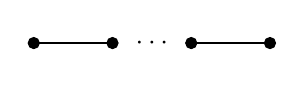
\begin{tikzpicture}
\filldraw (0,0) circle (2pt);
\filldraw (1,0) circle (2pt);
\node at (1.5,0) {$\cdots$};
\filldraw (2,0) circle (2pt);
\filldraw (3,0) circle (2pt);
\draw (0,0)--(1,0);
\draw (2,0)--(3,0);
\end{tikzpicture}
\end{center}
\end{definition}

\begin{example}
$\mathfrak{sl}_{n+1}$ corresponds to type $A_n$
\end{example}

\begin{definition}
Type $B_n$ corresponds to Dynkin diagram
\begin{center}
\begin{tikzpicture}
\filldraw (0,0) circle (2pt);
\filldraw (1,0) circle (2pt);
\node at (1.5,0) {$\cdots$};
\filldraw (2,0) circle (2pt);
\filldraw (3,0) circle (2pt);
\filldraw (4,0) circle (2pt);
\draw (0,0)--(1,0);
\draw (2,0)--(3,0);
\draw (3,2pt)--(4,2pt);
\draw (3,-2pt)--(4,-2pt);
\draw ($(3.5,0)+(-2pt,4pt)$)--($(3.5,0)+(2pt,0)$)--($(3.5,0)+(-2pt,-4pt)$);
\end{tikzpicture}
\end{center}
\end{definition}

\begin{example}
$\mathfrak{so}_{2n+1}$ corresponds to type $B_n$
\end{example}

\begin{definition}
Type $C_n$ corresponds to Dynkin diagram
\begin{center}
\begin{tikzpicture}
\filldraw (0,0) circle (2pt);
\filldraw (1,0) circle (2pt);
\node at (1.5,0) {$\cdots$};
\filldraw (2,0) circle (2pt);
\filldraw (3,0) circle (2pt);
\filldraw (4,0) circle (2pt);
\draw (0,0)--(1,0);
\draw (2,0)--(3,0);
\draw (3,2pt)--(4,2pt);
\draw (3,-2pt)--(4,-2pt);
\draw ($(3.5,0)+(2pt,4pt)$)--($(3.5,0)+(-2pt,0)$)--($(3.5,0)+(2pt,-4pt)$);
\end{tikzpicture}
\end{center}
\end{definition}

\begin{example}
$\mathfrak{sp}_{2n}$ corresponds to type $C_n$
\end{example}

\begin{definition}
Type $D_n$ corresponds to Dynkin diagram
\begin{center}
\begin{tikzpicture}
\filldraw (0,0) circle (2pt);
\filldraw (1,0) circle (2pt);
\node at (1.5,0) {$\cdots$};
\filldraw (2,0) circle (2pt);
\filldraw (3,0) circle (2pt);
\filldraw (4,1) circle (2pt);
\filldraw (4,-1) circle (2pt);
\draw (0,0)--(1,0);
\draw (2,0)--(3,0);
\draw (3,0)--(4,1);
\draw (3,0)--(4,-1);
\end{tikzpicture}
\end{center}
\end{definition}

\begin{example}
$\mathfrak{so}_{2n}$ corresponds to type $D_n$
\end{example}

\begin{definition}
Type $F_4$ corresponds to Dynkin diagram
\begin{center}
\begin{tikzpicture}
\filldraw (0,0) circle (2pt);
\filldraw (1,0) circle (2pt);
\filldraw (2,0) circle (2pt);
\filldraw (3,0) circle (2pt);
\draw (0,0)--(1,0);
\draw (2,0)--(3,0);
\draw (1,2pt)--(2,2pt);
\draw (1,-2pt)--(2,-2pt);
\draw ($(1.5,0)+(-2pt,4pt)$)--($(1.5,0)+(2pt,0)$)--($(1.5,0)+(-2pt,-4pt)$);
\end{tikzpicture}
\end{center}
\end{definition}

\begin{definition}
Type $G_2$ corresponds to Dynkin diagram
\begin{center}
\begin{tikzpicture}
\filldraw (0,0) circle (2pt);
\filldraw (1,0) circle (2pt);
\draw (0,0)--(1,0);
\draw (0,2pt)--(1,2pt);
\draw (0,-2pt)--(1,-2pt);
\draw ($(0.5,0)+(-2pt,4pt)$)--($(0.5,0)+(2pt,0)$)--($(0.5,0)+(-2pt,-4pt)$);
\end{tikzpicture}
\end{center}
\end{definition}

\begin{definition}
Type $E_6$ corresponds to Dynkin diagram
\begin{center}
\begin{tikzpicture}
\filldraw (0,0) circle (2pt);
\filldraw (1,0) circle (2pt);
\filldraw (2,0) circle (2pt);
\filldraw (3,0) circle (2pt);
\filldraw (4,0) circle (2pt);
\filldraw (2,1) circle (2pt);
\draw (0,0)--(1,0)--(2,0)--(3,0)--(4,0);
\draw (2,0)--(2,1);
\end{tikzpicture}
\end{center}
\end{definition}

\begin{definition}
Type $E_7$ corresponds to Dynkin diagram
\begin{center}
\begin{tikzpicture}
\filldraw (0,0) circle (2pt);
\filldraw (1,0) circle (2pt);
\filldraw (2,0) circle (2pt);
\filldraw (3,0) circle (2pt);
\filldraw (4,0) circle (2pt);
\filldraw (5,0) circle (2pt);
\filldraw (2,1) circle (2pt);
\draw (0,0)--(1,0)--(2,0)--(3,0)--(4,0)--(5,0);
\draw (2,0)--(2,1);
\end{tikzpicture}
\end{center}
\end{definition}

\begin{definition}
Type $E_8$ corresponds to Dynkin diagram
\begin{center}
\begin{tikzpicture}
\filldraw (0,0) circle (2pt);
\filldraw (1,0) circle (2pt);
\filldraw (2,0) circle (2pt);
\filldraw (3,0) circle (2pt);
\filldraw (4,0) circle (2pt);
\filldraw (5,0) circle (2pt);
\filldraw (6,0) circle (2pt);
\filldraw (2,1) circle (2pt);
\draw (0,0)--(1,0)--(2,0)--(3,0)--(4,0)--(5,0)--(6,0);
\draw (2,0)--(2,1);
\end{tikzpicture}
\end{center}
\end{definition}

\begin{remark}
The number in the subscript is the number of nodes. In particular, we have \par
$A_1=B_1=C_1$
\begin{center}

\begin{tikzpicture}
\filldraw (0,0) circle (2pt);
\end{tikzpicture}
\end{center}
$B_2=C_2$
\begin{center}
\begin{tikzpicture}
\filldraw (3,0) circle (2pt);
\filldraw (4,0) circle (2pt);
\draw (3,2pt)--(4,2pt);
\draw (3,-2pt)--(4,-2pt);
\draw ($(3.5,0)+(2pt,4pt)$)--($(3.5,0)+(-2pt,0)$)--($(3.5,0)+(2pt,-4pt)$);
\end{tikzpicture}
\end{center}
$D_3=A_3$
\begin{center}
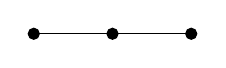
\begin{tikzpicture}
\filldraw (0,0) circle (2pt);
\filldraw (1,0) circle (2pt);
\filldraw (2,0) circle (2pt);
\draw(0,0)--(1,0)--(2,0);
\end{tikzpicture}
\end{center}
$D_2=A_1A_1$ \par
$E_3=A_2A_1$ \par
$E_4=A_4$
\begin{center}
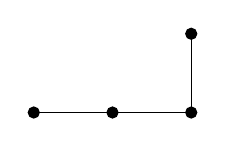
\begin{tikzpicture}
\filldraw (0,0) circle (2pt);
\filldraw (1,0) circle (2pt);
\filldraw (2,0) circle (2pt);
\filldraw (2,1) circle (2pt);
\draw (0,0)--(1,0)--(2,0);
\draw (2,0)--(2,1);
\end{tikzpicture}
\end{center}
$E_5=D_5$
\begin{center}
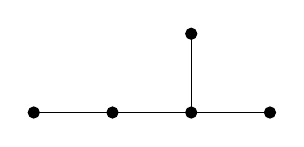
\begin{tikzpicture}
\filldraw (0,0) circle (2pt);
\filldraw (1,0) circle (2pt);
\filldraw (2,0) circle (2pt);
\filldraw (3,0) circle (2pt);
\filldraw (2,1) circle (2pt);
\draw (0,0)--(1,0)--(2,0)--(3,0);
\draw (2,0)--(2,1);
\end{tikzpicture}
\end{center}
\end{remark}

\begin{theorem}[Cartan-Killing classification]\label{Cartan-Killing classification}
The above Dynkin diagrams classifies simple Lie algebras
\end{theorem}

\begin{proof}
Consider the \textbf{admissible sets} of Euclidean space $V$, $A=\{v_1,\cdots,v_n\}$ of linearly independent unit vectors with $(v_i,v_j)\leq0$ and $4(v_i,v_j)^2\in \{0,1,2,3\}$ if $i\neq j$. Define Coxeter diagram $\Gamma_A$ for $A$  to have vertices $v_1,\cdots,v_n$, and $d_{ij}= 4(v_i,v_j)^2$ edges between $v_i$ and $v_j$ if $i\neq j$. Assume that $\Gamma_A$ is connected \par
\begin{enumerate}[leftmargin=*,label=\textbf{\alph*)}]
\item The number of vertices in $\Gamma_A$ joined by at least one edge is at most $|A|-1$ \par
$v=v_1+\cdots+v_n\neq 0$ satisfies $(v,v) =n+ 2\displaystyle\sum_{i<j}(v_i,v_j)>0$, thus $n >-\displaystyle\sum_{i<j}2(v_i,v_j) =\sum_{i<j}\sqrt{d_{ij}}\geq N$, where $N$ is the number of pairs $v_i,v_j$ such that $d_{ij}\geq 1$
\item The graph $\Gamma_A$ contains no cycles \par
The vectors in a cycle of $\Gamma_A$ form an admissible set which a contradicts a)
\item No vertex in $\Gamma_A$ has more than $3$ edges \par
Let $w$ be a vertex of $\Gamma_A$ with adjacent vertices $w_1,\cdots,w_k$, then $(w_i,w_j) = 0$ for $i\neq j$.  Let $U= \Span_{\mathbb R}(w_1,\cdots,w_k,w)$, and extend $\{w_1,\cdots,w_k\}$ to an orthonormal basis of $U$, say by adjoining $w_0$. Clearly $(w,w_0)\neq 0$ and $w=\displaystyle\sum^k_{i=0}(w,w_i)w_i$. Hence $1 = (w,w)= \displaystyle\sum^k_{i=0}(w,w_i)^2$, $\displaystyle\sum^k_{i=1}(w,w_i)^2<1$, $w$ has no more than $3$ edges
\item If $\Gamma_A$ has triple edge, then by c), the $\Gamma _A$ can only be $G_2$
\item Assume $\Gamma_A$ has a subgraph which is a line along $w_1,\cdots,w_n$, if we replace this subgraph with $w=w_1+\cdots+w_n$, then it is still an admissible set \par
$(w,w)=n+\displaystyle2\sum_{i=1}^{n-1}(w_i,w_{i+1})=n-(n-1)=1$, by d) any vertex $v$ has at most edges linked with one such $w_i$, hence $(v,w)=(v,w_i)$, this gives an admissible set
\item A branch point is a vertex having more than $2$ adjacent vertices, in this case, exactly $3$. $\Gamma_A$ has only one double edge, or only one branch point, or neither, but not both. Note that if $\Gamma_A$ has no brach points and double edges corresponds to $A_n$ \par
If $\Gamma_A$ has two double edges between $w_1,w_2$ and $v_1,v_2$, then they can be linked through a line, by e), we can collapse it into a single vertex, but this will contradict c)
\item If $\Gamma_A$ has a subgraph which is a line through $w_1,\cdots,w_n$, let $w=\sum iw_i$, then $(w,w)=\dfrac{n(n+1)}{2}$
\item If $\Gamma_A$ has a double edge, then $\Gamma_A$ is $F_4$ or $B_n$ \par
By f) we know $\Gamma_A$ is a line through $v_1,\cdots,v_p,w_q,\cdots,w_1$, $q\geq p\geq1$ with single edges except $v_p,w_q$, let $v=\sum iv_i$, $w=\sum iw_i$, then
\[(v,w)^2=(pv_p,qw_q)^2=\frac{p^2q^2}{2}\]
Since $v,w$ are linearly independent, by Cauchy Schwarz inequality, we have
\[\frac{p^2q^2}{2}=(v,w)^2<(v,v)(w,w)=\frac{p(p+1)q(q+1)}{4}\]
Which implies $(p-1)(q-1)<2$, thus if $p=1$, then $q$ can be any positive interger, giving $B_n$, if $p=2$, then $q=2$, giving $F_4$
\item If $\Gamma_A$ has a branch point, then $\Gamma_A$ is $D_n$ or $E_6,E_7,E_8$ \par
$\Gamma_A$ is has three branch lines $v_1,\cdots,v_p,x$ and $w_1,\cdots,w_q,x$ together with $z_1,\cdots,z_r,x$, $p\geq q\geq r$, let $v=\sum iv_i$, $w=\sum iw_i$, $z=\sum iz_i$ which are pairwise orthogonal, $\hat v,\hat w,\hat z$ be normalized vectors of $v,w,z$, and consider $U=\Span_{\mathbb R}(v,w,z,x)=\Span_{\mathbb R}(\hat v,\hat w,\hat z,x_0)$, where $x_0$ is a unit vector orthogonal to $v,w,z$, then $(x,x_0)\neq0$
\[1=(x,x)=(x,\hat v)^2+(x,\hat w)^2+(x,\hat z)^2+(x,x_0)^2\]
Thus by g)
\[\frac{2p^2}{4p(p+1)}+\frac{2q^2}{4q(q+1)}+\frac{2r^2}{4r(r+1)}<1\]
Hence
\[\frac{1}{1+p}+\frac{1}{1+q}+\frac{1}{1+r}>1\]
and we know that
\[\frac{1}{1+p}\leq\frac{1}{1+q}\leq\frac{1}{1+r}\leq\frac{1}{2}\]
Hence $r=1$
\[\frac{1}{1+p}+\frac{1}{1+q}>\frac{1}{2}\]
If $q=1$, then $p$ can be any positive integer, giving $D_n$, if $q=2$, then $p$ can only be $2,3$ or $4$, giving $E_6,E_7,E_8$
\end{enumerate}
\end{proof}

\begin{lemma}
$(V,\Delta)$ be a irreducible root system, $\Delta^+$ be a set of positive roots and $S=\{\alpha_1,\cdots,\alpha_n\}$ be its base, then there exists unique highest root $\gamma\in\Delta$, meaning $\gamma+\alpha_i\in\Delta,\forall\alpha_i\in S$
\end{lemma}

\begin{definition}
Let $(V,\Delta)$ be a irreducible root system, $\Delta^+$ be a set of positive roots, $S=\{\alpha_1,\cdots,\alpha_n\}$ be its base, and $\gamma$ its unique highest root, the extended Dynkin diagram is the usual Dynkin diagram adding $\alpha_0=-\gamma$, the number of bonds for each two nodes and direction are still defined as before. Finally, suppose $-\alpha_0=\sum n_i\alpha_i$, then lebel $\gamma$ with \textcircled{\small 1}, and label node $\alpha_i$ with $n_i$
\end{definition}

\begin{lemma}
If the following part of the extended Dynkin diagram
\begin{center}
\begin{tikzpicture}
\filldraw [black] (0,0) circle (2pt);\coordinate (a) at (0,0);\node[below] at (a){$a$};
\filldraw [black] (-1,0) circle (2pt);\coordinate (b) at (-1,0);\node[below] at (b){$b$};
\filldraw [black] (-2,0) circle (2pt);\coordinate (c) at (-2,0);
\filldraw [black] (-3,0) circle (2pt);\coordinate (d) at (-3,0);
\filldraw [black] (1,0) circle (2pt);\coordinate (e) at (1,0);\node[below] at (e){$b$};
\filldraw [black] (2,0) circle (2pt);\coordinate (f) at (2,0);
\filldraw [black] (3,0) circle (2pt);\coordinate (g) at (3,0);
\filldraw [black] (0,1) circle (2pt);\coordinate (h) at (0,1);\node[right] at (h){$c$};
\node at (-1.5,0){$\cdots$};\node at (1.5,0){$\cdots$};
\draw[-] (a)--(b);\draw[-] (c)--(d);\draw[-] (a)--(e);\draw[-] (f)--(g);\draw[-] (a)--(h);
\end{tikzpicture}
\end{center}
We have $2a=b+c+d$
\end{lemma}

\begin{example}
Consider the classical root system $D_n$, $\Delta^+=\{e_i\pm e_j|i<j\}$, $S=\{e_1-e_2,\cdots,e_{n-1}-e_n,e_{n-1}+e_n\}$, then $\gamma=e_1+e_2$, its usual Dynkin diagram is
\begin{center}
\begin{tikzpicture}
\filldraw [black] (0,0) circle (2pt);\coordinate (a) at (0,0);
\filldraw [black] (-1,0) circle (2pt);\coordinate (b) at (-1,0);
\filldraw [black] (-2,0) circle (2pt);\coordinate (c) at (-2,0);
\filldraw [black] (-3,0) circle (2pt);\coordinate (d) at (-3,0);
\filldraw [black] (-4,0) circle (2pt);\coordinate (e) at (-4,0);
\filldraw [black] (1,1) circle (2pt);\coordinate (f) at (1,1);
\filldraw [black] (1,-1) circle (2pt);\coordinate (g) at (1,-1);
\node at (-1.5,0){$\cdots$};
\draw[-] (a)--(b);\draw[-] (c)--(e);\draw[-] (a)--(f);\draw[-] (a)--(g);
\end{tikzpicture}
\end{center}
So its extended Dynkin diagram is
\begin{center}
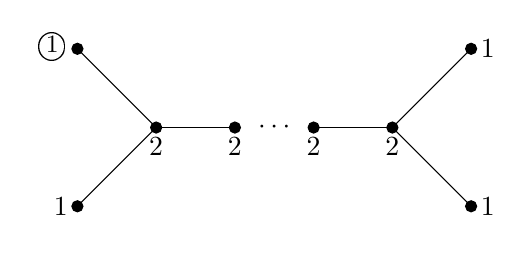
\begin{tikzpicture}
\filldraw [black] (0,0) circle (2pt);\coordinate (a) at (0,0);\node[below] at (a){$2$};
\filldraw [black] (-1,0) circle (2pt);\coordinate (b) at (-1,0);\node[below] at (b){$2$};
\filldraw [black] (-2,0) circle (2pt);\coordinate (c) at (-2,0);\node[below] at (c){$2$};
\filldraw [black] (-3,0) circle (2pt);\coordinate (d) at (-3,0);\node[below] at (d){$2$};
\filldraw [black] (-4,-1) circle (2pt);\coordinate (e) at (-4,-1);\node[left] at (e){$1$};
\filldraw [black] (1,1) circle (2pt);\coordinate (f) at (1,1);\node[right] at (f){$1$};
\filldraw [black] (1,-1) circle (2pt);\coordinate (g) at (1,-1);\node[right] at (g){$1$};
\filldraw [black] (-4,1) circle (2pt);\coordinate (h) at (-4,1);\node[left] at (h){\textcircled{\small 1}};
\node at (-1.5,0){$\cdots$};
\draw[-] (a)--(b);\draw[-] (c)--(d);\draw[-] (d)--(e);\draw[-] (a)--(f);\draw[-] (a)--(g);\draw[-] (d)--(h);
\end{tikzpicture}
\end{center}
\end{example}



\end{document}